\chapter[Forward-Looking Sonar Image Classification]{Forward-Looking Sonar \newline Image Classification}
\label{chapter:sonar-classification}

Image classification is one of the fundamental problems in Computer Vision and Robot Perception. It is also one of the most basic problems, as many techniques have image classification sub-tasks.

The Image Classification is the task given an image, classify it as one of $C$ predefined classes. This task is commonly implemented with ML algorithms, as it directly maps to the training of a classifier on image inputs.

In this chapter we perform a comprehensive evaluation of image classification algorithms on FLS images, including classic techniques like template matching as well as advanced classification algorithms. We wish to investigate the following research questions:

\begin{itemize}
	\item Can we use feature learning methods on FLS images?
	\item Can object recognition be performed with high accuracy and low number of assumptions on object shape, shadow or highlight?
    \item Can we use deep neural networks to classify FLS images on embedded systems?
\end{itemize}

\section{Related Work}

Image classification methods are typically embedded into a bigger system, such as object detection or automatic target recognition systems. In this literature review we focus on classification as a separate problem, as the bottleneck for a good detection or recognition system is usually classifier performance. Without a good classification algorithm, high performance on object detection or target recognition is not possible.

The most basic classification method for Sonar images is to use template matching, which is a specific way of computing similarity between two images. If a labeled set of template images\footnote{This is just a set of same-size images where each is labeled with a corresponding class.} is available, then a given test image can be classified by computing the similarity with each template image and finding the "most similar" image, and outputting the class label of that image. This method is similar to a k-nearest neighbours (KNN) classifier with $k = 1$ and using the similarity as a feature space.

Two similarity computation techniques are popular \cite{gonzalezDIP2006}, namely normalized cross-correlation and sum of squared differences.

Cross-correlation, computes the correlation $\sum I \star T$ between an image $I$ and template image $T$, where $\star$ is component-wise multiplication. As the correlation is unbounded, a normalized version is preferred. $I$ and $T$ are normalized by subtracting the mean and dividing by the standard deviation, which leads to the operation in Eq \ref{sic:ccSimilarityEq}:
\vspace*{1em}
\begin{equation}
	S_{CC}(T, I) = \frac{\sum (I - \bar{I}) \sum (T - \bar{T})}{\sqrt{\sum (I - \bar{I})^2 \sum (T - \bar{T})^2}}
	\label{sic:ccSimilarityEq}
\end{equation}

The normalized cross-correlation produces a number in the $[-1, 1]$ range. Note that this version of cross-correlation is slightly different from the one used to perform object detection, as the template is not slid over the image, as the test and template images are assumed to be the same size. In order to perform classification, the template with highest normalized cross-correlation is selected.

Sum of squared differences similarity (SQD) just computes the average square of the difference between the test image $I$ and the template image $T$ (Eq \ref{sic:sqdSimilarityEq}). The idea of SQD is to find the template that is most similar to the test image in terms of raw euclidean distance between pixels.
\vspace*{1em}
\begin{equation}
	S_{SQD}(T, I) = n^{-1} \sum (I - T)^2
	\label{sic:sqdSimilarityEq}
\end{equation}

Reed et al. \cite{reed2004automated} propose a shape matching approach for image classification. A training dataset is generated by using CAD models to generate synthetic sidescan sonar images for matching. A test image is classified by first detecting mine-like objects (Cylinder, Sphere and Cone) with a Markov Random Field model and the shadow and highlight are segmented. The shadow shape is then matched with one in the training set by means of the minimum Hausdorff distance.

As one match is produced per class, the authors combine a match from each of the three classes using Fuzzy Logic. This method is quite complex as multiple manually engineered equations are required, with little theory to support them.

In order to improve the robustness of their results, Reed et al. \cite[-7em]{reed2004automated} use Dempster-Shafer information theory to fuse predictions from multiple views. In single-view classification, their method obtains $90 \%$ correct classifications with $50 \%$ false alarms produced by the detection/segmentation step of their method.
In multi-view classification, a Cylinder can be classified with $93.9 \%$ accuracy, while a Cone produces $67.5 \%$ accuracy, and a Sphere with $98.3 \%$ accuracy.
The results are not impressive for such simple shaped objects, as multiple views are required to obtain a high accuracy classifier, but still the Cone object is poorly classified.

Fawcett et al. \cite{fawcett2007computer} use engineered features based on shadow and highlight shape to classify mine-like objects (Cylinder, Cone, Truncated Cone) in SAS images. Shadow/highlight segmentation is required. 38 different features are used for shadows, while 57 features are used for highlights. The authors only provide vague information about the features they used, namely "profiles", perimeter, area, pixel statistics of the regions. A  Radial Basis Function classifier with a Gaussian Kernel

Additional features are computed with Principal Component Analysis (PCA), by projecting each image into the first 5 principal components, which produces an additional 5-dimensional feature vector. Different combination of features are tested. $90 \%$ classification accuracy is obtained with shadow, highlight, and PCA features. Other combinations of features performed slightly worse, but notably shadow-only features obtained considerably worse accuracy (around $40 \%$). An interesting observation made in this work is that using the normalized image pixels as a feature vector obtains almost the same classification performance as the more complex set of features.

Myers and Fawcett \cite{myers2010template} proposed the Normalized Shadow-Echo Matching (NSEM) method for object detection in SAS images. NSEM first requires to segment the sonar image into bright echo, echo, background, shadow and dark shadow. Fixed values are assigned to each segmentation class (in the range $[-1, 1]$).
Then similarity is computed with a custom correlation function shown in Eq. \ref{sic:myersFawcettSimilarity}, where $I$ and $T$ are the segmented and post-processed test and template images, $I \otimes T = \sum T \star I$ is the standard cross-correlation operator, and $I_E$/$T_E$ are the highlight components of the corresponding images, and $I_S$/$T_S$ are the shadow components. The bar operation inverts the image, setting any non-zero element to zero, and any zero value to one.
\vspace*{1em}
\begin{equation}
	f(T, I) = \frac{I \otimes T_E}{1 + I_E \otimes \bar{T}_E} + \frac{I \otimes T_S}{1 + I_S \otimes \bar{T}_S}
	\label{sic:myersFawcettSimilarity}
\end{equation}

The final classification is performed by outputting the class of the template with the highest similarity score as given by Eq. \ref{sic:myersFawcettSimilarity}. This method can also be used as an object detector by setting a minimum similarity threshold to declare a detection.

This method was tested on a 3-class dataset of MLOs, namely Cylinder, Cone, Truncated Cone, and Wedge shapes. Target templates were generated using a SAS simulator, adding multiple views by rotating the objects. Objects are correctly classified with accuracies in the range $97-92 \%$, which is slightly higher than the reported baseline using normalized cross-correlation with the raw image ($92-62 \%$) and segmented images ($95-81 \%$). This method performs quite well as reported, but it requires a segmentation of the input image, which limits its applicability to marine debris.

Sawas et al. \cite{sawas2010cascade} \cite[1em]{sawas2012cascade} propose boosted cascades of classifiers for object detection in SAS images. This method can also be used for classification, as its core technique (Adaboost) is a well-known ML classification framework . Haar features are quite similar to the shadow-highlight segmentation present in typical sonar images, which is that motivates their use. Haar features have the additional advantage that they can be efficiently computed using summed-area tables.

A boosted cascade of classifiers \cite[1em]{bishop2006pattern} is a set of weak classifiers \footnote[][1em]{Classifiers with low accuracy, but computationally inexpensive} that are stacked in a cascade fashion. The basic idea originally introduced by Viola-Jones \cite[2em]{viola2001rapid} for face detection is that weak classifiers at the beginning of the cascade can be used to quickly reject non-face windows, while classifiers close to the end of the cascade can concentrate on more specific features for face detection. AdaBoost is then used to jointly train these classifiers.
This structure produces a very efficient algorithm, as the amount of computation varies with each stage and depth in the cascade (deep classifiers can use more features, while shallow classifiers can use less), but fast to compute features are required, as feature selection is performed during training.

Sawas et al. proposes an extension to the classic Haar feature, where a long shadow area with a small highlight is used as a Haar feature, matching the signature from the MLOs that are used as targets. On a synthetic dataset with Manta, Rockan and Cylinder objects, the authors obtain close to $100 \%$ accuracy for the Manta, but Rockan and Cylinder only obtain around $80-90 \%$ accuracy.
On a semi-synthetic dataset with the same objects, results are slightly different, with Manta saturating at $97 \%$ accuracy, while the other objects obtain $93-92 \%$ accuracy. When used as an object detector, this method is very fast but it suffers from a large amount of false positives. The use of Haar features also makes it quite specific to MLOs, as their unique shadow-highlight pattern is not produced by marine debris.

Dura et al. \cite{dura2011image} surveys techniques for detection and classification of MLOs in sidescan sonar images. She describes two principal types of features for MLO classification: shape and gray-level.

Shape features consist of geometric characteristics from shadow or highlight regions. It is mentioned that Man-made objects project regular and predictable shadow and highlight regions. Shape features include: area, elongation, circularity, orientation, eccentricity, rectangularity, number of zero crossings of the curvature function at multiple scales. Many of these features are computed as functions of the central moments of order $p + q$:
\vspace*{1em}
\begin{equation}
	\mu_{pq} = \sum_x \sum_y (x - x_g)^p (y - y_g)^q I(x, y)
\end{equation}

Where $(x_g, y_g)$ is the centre of mass of the region and $I(x, y)$ is the region pixels. 

Gray-level features are statistics of the shadow and highlight regions, and are useful for low resolution images. Such features consider: shadow/highlight mean and variance, ratios between shadow and highlight, shadow vs background, and highlight vs background. These ratios are typically computed from means across each kind of region. While only a qualitative comparison is provided, the only quantitative results correspond to the ones published in each work.

All of these features require segmentation between shadow, highlight and background. This is a considerable disadvantage, as marine debris does not always possess a shadow, due to the small object size.
This work also briefly compares single and multi-view classification. Using multiple views usually reduces classification uncertainty, but this process introduces additional complexity due to the choice of fusion algorithm and more complex features.

Fandos and Zoubir \cite[-2em]{fandos2011optimal} provides a numerical comparison of shape and statistical shadow/highlight features on SAS images. Cylindrical, Spherical and Background objects were considered. Normalized central moments obtain $90-80 \%$ accuracy, while PCA features with three principal components obtains close to $80 \%$ accuracy.

Statistical features on shadow and highlight saturate to $70 \%$ accuracy across many combinations. Brute force combination of all features produces overfitting due to the curse of dimensionality. An empirical obtained optimal feature vector formed by shadow and highlight shape features, two normalized central moments, the second principal component, the shadow-background/shadow-highlight/highlight-background scale Weybull parameters, and the segmentation quality parameter.
This feature vector produces $95 \%$ classification accuracy, which is the best result in this work. But such a complicated feature vector does not necessarily generalize to other objects, specially when considering the variability of marine debris shape.

Fandos et al. \cite{fandos2012sparse} compare the use of sparse representations versus a Linear Discriminant Analysis (LDA) classifier. Features consist of the raw SAS image, a segmented SAS image, the fourier coefficients of the shadow, 50 principal components obtained from PCA applied to the shadow, and 10-th order normalized central moments of the segmented shadow. Feature selection was performed with sequential forward floating search and a optimal feature set was obtained, it contains a subset of the previously mentioned features.

$95 \%$ classification accuracy can be obtained on the optimal feature set, but the same features after a sparse representation has been obtained perform considerably worse, with differences up to $25 \%$ less absolute accuracy. As mentioned in the similar previous work, it is not clear how these features would generalize to different objects, and these features seem too specific to MLOs.

Hurtos et al. \cite{hurtos2013automatic} uses normalized cross-correlation template matching to detect the four corners of a chain link in a FLS image (from an ARIS Explorer 3000). This application is the one that can be considered closest to this work, as detecting and classifying chain link corners is a considerably more hard problem than MLO classification.
Templates are selected by cropping images at each of the four corners of the chain link, and rotations are introduced in order to generate a bigger template set. Results over three datasets shows classification performance in the range $92-84 \%$ accuracy. While this result is appropriate for the chain following task, it is quite weak from a classification point of view, as template matching does not seem to produce robust results. Authors of this work had to use mosaicing by averaging three frames in order to reduce noise in the image, which shows that using the raw FLS image with template matching could potentially reduce classification performance.

In the same line as the previous work, Ferreira et al. \cite{ferreira2014improving} also use mosaicing to improve classification performance in FLS images (obtained from a BlueView P450-130). A classification algorithm using morphological and echo/background ratios is used. Using this classifier with raw data produces $40 \%$ correct classifications, while using mosaiced images produces $38.4 \$$ accuracy, but the number of misclassifications is reduced.

Barngrover et al. \cite{barngrover2015semisynthetic} evaluate the effect of using semi-synthetic data versus real data. Their motivation is to use ML classification algorithms that require several thousands of data points in order to generalize well. They generate semi-synthetic data by segmenting the object out of a real image and placing it in new different backgrounds.

The authors use a boosted cascade of weak classifier (same as Sawas et al.) with Haar and Local Binary Pattern (LBP) features. For Haar features, classifiers that were trained on real data have an accuracy advantage of around $3 \%$ over classifiers that were trained on semi-synthetic data, but the classifiers on real data saturate at $93-92 \%$ correct classification.
For LBP features, the difference is more drastic, as using a classifier trained on real data has a $20 \%$ accuracy advantage over using synthetic data. A classifier trained on real data obtains close to $90 \%$ accuracy, while synthetic classifiers obtain $70 \%$. Some specific configurations of semi-synthetic data generation can improve accuracy to the point of a $6 \%$ difference versus the real classifier.

David Williams \cite{williams2016underwater} performs target classification in SAS images using a CNN with sigmoid activations. His dataset contains MLO-like objects for the positive class (cylinders, wedges, and truncated cones), while the negative class contain distractor objects like rocks, a washing machine, a diving bottle, and a weighted duffel bag, with a training set of over 65K images. Three binary classification experiments are performed, namely fully positive vs negative class, truncated cones vs rocks, and MLO mantas vs truncated cones as they are visually similar. The ROC curve and the area under the curve (AUC) are used as  evaluation metrics. In all experiments a 10-layer convolutional neural network obtained better results than the baseline (a relevance vector machine).

David Williams \cite[-1em]{williams2018underwater} has also explored transfer learning for SAS images. Using the previously mentioned networks trained on SAS data, each network was fine-tuned on new data of cylindrical objects versus clutter, and evaluated on a previously unseen dataset, showing that the fine-tuning process improves classification performance in terms of the AUC. A more interesting results is for transfer learning across different sonar sensors, where a CNN is trained on one SAS sensor, and fine-tuned in another. The fine-tuning process indeed shows improvements in AUC, even as less samples per class are available.
This work does not use a robust method to decide the network architecture, as a model with less parameters could perform better. No baselines are provided, which makes interpreting the results difficult.

Zhu et al. \cite{zhu2017deeplearning} uses AlexNet pre-trained on the ImageNet dataset to extract features from sidescan sonar images, and use them for object classification with an SVM. CNN features obtain up to $95 \%$ accuracy, outperforming Local Binary Patterns and Histogram of Oriented Gradient features when used with an SVM classifier. The dataset contains 35 sonar images, containing objects of interest over binary classes (targets/no targets), but no more detail about object classes is provided.

K\"ohntopp et al. \cite{kohntopp2017seafloor} provide results for seafloor classification in SAS images. Their dataset contains three seafloor classes: flat, rocky and ripples. They compare different handcrafted features, namely fractal dimension, wavelets, anisotropy and complexity, texture features, lacunarity, and a combination of these features, versus a Convolutional Neural Network that they designed. Two classic classifiers are evaluated, including a SVM and Naive Bayes.

The CNN outperforms all other handcrafted features with both classifiers, obtaining an accuracy of $98.7 \%$. Handcrafted features' performance varies, with the best being the fractal dimension with an SVM classifier ($97.7 \%$) and wavelets features ($94.9 \%$). A CNN outperforms an SVM by $1 \%$.
There is still many ways to improve these results, like including additional regularization (Batch Normalization) and fine-tuning the network architecture, but these results show that using CNNs on sonar data is promising.

Buss et al. \cite{buss2018hand} compare hand-crafted features from a feed-forward neural network versus feature learning by a convolutional neural network on data from a Cerberus active diver detection sonar developed by Atlas Electronics. Their dataset contains 490 samples of divers, and 114K non-diver or background samples. Surprisingly, the feed-forward neural network using hand-crafted features outperforms both a shallow CNN and VGG, obtaining a higher area under the ROC curve ($0.99 - 0.93$) and reducing false positives by $89 \%$. This result can be explained by the large imbalance between targets and non-targets, and additional domain knowledge introduced by the feature engineering process.

\subsection{Discussion}

Most applications of object recognition/classification in underwater domains correspond to mine-like objects. While it is questionable that large parts of the literature in this topic are devoted to pseudo-military research, there are better arguments about why this is a big problem.

Mine-like objects have simple geometrical shapes, namely Spheres, Cylinders, Cones, Truncated Cones, etc. This simplifies the development of recognition algorithms but these simplifications are not free, they usually make implicit assumptions. For example, using template matching can be done with templates that match certain views of the object, and an assumption is made that other views are not important for generalization. Enumerating all views of an object is not always possible.

Datasets used for MLO detection and classification are typically collected by military organizations and such data is most of the time classified\footnote{Information that is restricted from public access because of confidentiality, typically regulared by law.}. This hinders the development of the field, as only people in military research centers or with security clearance access can effectively perform experiments and advance the field. This is in contrast with the "open" policy of the Machine Learning community, where Datasets and Source Code are routinely shared and used as standard benchmarks. Machine Learning moves at a faster pace precisely because of their openness.

Moving into specific issues with classification algorithms for sonar images. All methods based on template matching suffer from severe disadvantages.

Using templates make implicit assumptions on object shape. Given a fixed set of templates, only a finite number of variations of the object can be modeled. Deciding which templates to use in order to detect/classify a set of objects is an open problem. For mine-like objects, typical choices are several views of each object that are synthetically generated, which alleviates the problem.

Each template's pixels could be considered as parameters in a ML classification algorithm. Using a large number of templates to classify an object could potentially be subject to overfitting, as model capacity increases and there is a higher chance than one of the templates produces a misclassified match.

Many methods require a segmentation of the image/template into shadow/highlight/background. From a ML point of view, this can be considered as regularization, as the number of free parameters is reduced by constraining them. For example, setting background pixels in segmented templates to zero reduces the effect of background. Segmenting sonar images is not trivial and it is a cumbersome part of the process, as it adds additional complexity that might not be required.

If the template and the object in a test image do not align, then the similarity will be low and classification will fail. To alleviate this problem it is typical to perform data augmentation by translating templates, introducing a small degree of translation invariance. But as mentioned before, increasing the number of templates could potentially lead to overfitting.

As a general overview of template matching accuracy, it is notable that most reviewed methods do not obtain accuracies higher than $95 \%$, with only some selected method obtaining higher accuracies, but never approaching $99 \%$. This pattern also supports our argument of mild overfitting, as the methods do not seem to generalize well and their accuracies quickly saturate.

About engineered features, they also suffer from some drawbacks. Many handcrafted features have no interpretation. For example, the fractal dimension, while having a physical meaning, does not necessarily have an interpretable meaning as a feature for image classification. Same can be said about Fourier or Wavelet features, as they are high dimensional and a learning algorithm can learn to overfit them.

Engineered features also suffer from generalization problems. While shadow and highlight geometric features seem to work for simple shaped objects like MLOs, they might fail to generalize over different objects, specially if their shapes are more complex. There is no reason that features that work well for MLOs will work well for marine debris.

It is well known that feature learning generally outperforms most kinds of feature engineering \cite{sharif2014cnn}. While it is not in question if learning features will outperform most engineered features, it is unknown by how much and how applicable is feature learning for the purpose of marine debris classification.

In the context of marine debris, we have observed that in our datasets, most marine debris-like objects have considerable differences with underwater mines that are relevant for classification:

\begin{itemize}
	\item In some cases, shape is not predictable. For example a plastic bottle might be crushed or deformed and his shape would be completely different than expected. In contrast, underwater mines are not typically deformed and they are designed to sustain water column pressure.
	\item MLOs have mostly convex shapes, while marine debris can have shapes with concave parts. This has the effect of producing strong reflections in the sonar image, and consequentially a much stronger viewpoint dependence. Simply, objects look quite different in the sonar image if you rotate them.
	\item Since the shape of MLOs is predictable and with a low intra/inter-class variation, the acoustic shadows that they produce are also predictable, and many methods exploit this property in order to do classification and detection. Marine debris does not have a predictable shadow shape as the object can be in any pose.
    \item Marine debris is usually much more small in physical size than MLOs, and in some cases marine debris does not produce acoustic shadows, which implies that only highlight information has to be used for classification.
\end{itemize}

\section{Classification using Convolutional Neural Networks}

In this section we describe our approach to classify FLS images with a Convolutional Neural Network. As most neural network architectures are designed for color images, we are forced to design our own architectures to fit the complexity and requirements of sonar data.

There are multiple hyper-parameters that must be tuned in order to obtain a proper neural network architecture. We take a simplified approach. We design several basic neural network modules that are "stacked" in order to build a more complex network. We let all modules inside a network to share the same set of hyper-parameters, and introduce a depth hyper-parameter, which is the the number of stacked modules on the network.

Modules that we use are shown in Fig. \ref{sic:basicModules}. We now describe the modules and their hyper-parameters:

\begin{description}
	\item[Classic Module] \hfill \\
		This is the most common module use by CNNs, starting from LeNet \cite[-4em]{lecun1998gradient}. It consists of one convolution layer followed by a max-pooling layer. Hyper-parameters are the number of filters $f$ and the size of the convolutional filters $s$. In this work we set $s = 5 \times 5$. This module is shown in Figure \ref{sic:basicModules}a.
		
	\item[Fire Module] \hfill \\
		The Fire module was introduced by Iandola et al. \cite{iandola2016squeezenet} as part of SqueezeNet.The basic idea of the Fire module is to use $1 \times 1$ convolutions to reduce the number of channels and $3 \times 3$ convolutions to capture spatial features. This module is shown in Figure \ref{sic:basicModules}b. The initial $1 \times 1$ convolution is used to "squeeze" the number of input channels, while the following $1 \times 1$ and $3 \times 3$ convolutions "expand" the number of channels.
		A Fire module has three hyper-parameters, the number of squeeze filters $s_{11}$, the number of expand $1 \times 1$ filters $e_{11}$, and the number of expand $3 \times 3$ filters $e_{33}$.
		
	\item[Tiny Module] \hfill \\
		The Tiny module was designed as part of this thesis. It is a modification of the Fire module, removing the expand $1 \times 1$ convolution and adding $2 \times 2$ Max-Pooling into the module itself. The basic idea of these modifications is that by aggressively using Max-Pooling in a network, smaller feature maps require less computation, making a network that is more computationally efficient. This module is shown in Figure \ref{sic:basicModules}c.
		The Tiny module has one hyper-parameter, the number of convolutional filters $f$, which is shared for both $1 \times 1$ and $3 \times 3$ convolutions.
		
	\item[MaxFire Module] \hfill \\
	This is a variation of the Fire module that includes two Fire modules with the same hyper-parameters and one $2 \times 2$ Max-Pooling inside the module. It is shown in Figure \ref{sic:basicModules}d and has the same hyper-parameters as a Fire module.
\end{description}
\vspace*{-1em}
\begin{figure*}[t]
	\centering
	\subfloat[Classic Module]{
		\begin{tikzpicture}[style={align=center, minimum width=2.2cm}]
		\node (E) {\scriptsize Input};
		\node[draw, above=1em of E] (D) {\scriptsize Conv2D($f$, $5 \times 5$)};
		\node[draw, above=1em of D] (C) {\scriptsize Max-Pool($2 \times 2$)};
		\node[draw, above=1em of C] (B) {\scriptsize Batch Norm};
		\node[above=1em of B] (A) {\scriptsize Output};
		\draw[-latex] (B) -- (A);
		\draw[-latex] (C) -- (B);
		\draw[-latex] (D) -- (C);
		\draw[-latex] (E) -- (D);
		\end{tikzpicture}
	}
	\subfloat[Fire Module]{
		\begin{tikzpicture}[style={align=center, minimum height=0.4cm, minimum width = 1.5cm}]
		
		\node[] (dummy) {};
		\node[draw, below=1em of dummy](B) {{\scriptsize Conv2D($s_{11}$, $1 \times 1$)}};
		\node[draw, left=0.25em of dummy] (C) {{\scriptsize Conv2D($e_{33}$, $3 \times 3$)}};
		\node[draw, right=0.25em of dummy] (D) {{\scriptsize Conv2D($s_{33}$, $1 \times 1$)}};
		\node[draw, above=1em of dummy](CONC) {{\scriptsize Merge}};
		\node[draw, above=1em of CONC](BN) {{\scriptsize Batch Norm}};
		\node[above=1em of BN] (O) {\scriptsize Output};
		\node[below=1em of B] (I) {\scriptsize Input};
		\draw[-latex] (B) -- (C);
		\draw[-latex] (C) -- (CONC);
		\draw[-latex] (B) -- (D);
		\draw[-latex] (D) -- (CONC);
		\draw[-latex] (I) -- (B);
		\draw[-latex] (BN) -- (O);
		\draw[-latex] (CONC) -- (BN);
		\end{tikzpicture}
	}	
	\subfloat[Tiny Module]{
		\begin{tikzpicture}[style={align=center, minimum height=0.4cm, minimum width = 2.3cm}]
		\node (I) {\scriptsize Input};
		\node[draw, above=1em of I] (A) {{\scriptsize Conv2D($f$, $3 \times 3$)}};
		\node[draw, above=1em of A] (B) {{\scriptsize Conv2D($f$, $1 \times 1$)}};
		\node[draw, above=1em of B](BN) {{\scriptsize Batch Norm}};
		\node[draw, above=1em of BN] (C) {{\scriptsize Max-Pool($2 \times 2$)}};
		\node[above=1em of C] (O) {\scriptsize Output};
		\draw[-latex] (A) -- (B);
		\draw[-latex] (C) -- (O);
		\draw[-latex] (I) -- (A);
		\draw[-latex] (B) -- (BN);
		\draw[-latex] (BN) -- (C);
		\end{tikzpicture}
	}
	\subfloat[MaxFire Module]{
		\begin{tikzpicture}[style={align=center, minimum height=0.4cm, minimum width = 2.0cm}]
		\node (I) {\scriptsize Input};
		\node[draw, above=1em of I] (A) {{\scriptsize Fire($s, e, e$)}};
		\node[draw, above=1em of A] (B) {{\scriptsize Fire($s, e, e$)}};
		\node[draw, above=1em of B](BN) {{\scriptsize Batch Norm}};
		\node[draw, above=1em of BN] (C) {{\scriptsize Max-Pool($2 \times 2$)}};
		\node[above=1em of C] (O) {\scriptsize Output};
		\draw[-latex] (A) -- (B);
		\draw[-latex] (C) -- (O);
		\draw[-latex] (I) -- (A);
		\draw[-latex] (B) -- (BN);
		\draw[-latex] (BN) -- (C);
		\end{tikzpicture}
	}
	\vspace*{0.2cm}
	\caption[Basic Convolutional Modules]{Basic Convolutional Modules that are used in this Chapter}
	\label{sic:basicModules}
\end{figure*}

All modules in Figure \ref{sic:basicModules} use ReLU as activation. We designed four kinds of neural networks, each matching a kind of module. Networks are denominated as ClassicNet, TinyNet and FireNet. While FireNet is quite similar to SqueezeNet, we did not want to use that name as it refers to a specific network architecture that uses the Fire module. Our FireNet uses the MaxFire module instead.

To build ClassicNet, we stack $N$ Classic modules and add two fully connected layers as classifiers. This corresponds to a configuration FC(64)-FC(C), where $C$ is the number of classes. The first fully connected layer uses a ReLU activation, while the second uses a softmax in order to produce class probabilities. This architecture can be seen in Figure \ref{sic:classicNet}.

FireNet is built in a similar way, but differently from ClassicCNN. This network contains an initial convolution to "expand" the number of available channels, as sonar images are single channel. Then $N$ MaxFire modules are stacked. Then a final convolution is used, in order to change the number of channels to $C$. Then global average pooling \cite{lin2013network} is applied to reduce feature maps from any size to $1 \times 1 \times C$. FireNet is shown in Figure \ref{sic:fireNet}.
TinyNet is similarly constructed, but it does not have a initial convolution. It contains a stack of $n$ Tiny modules with a final $1 \times 1$ convolution to produce $C$ output channels. Global average pooling is applied and a softmax activation is used to produce output class probabilities. TinyNet is shown in Figure \ref{sic:tinyNet}.

Both FireNet and TinyNet do not use fully connected layers for classification, and instead such layers are replaced by global average pooling and a softmax activation. This is a very different approach, but it is useful as it reduces the number of learning parameters, reducing the chance of overfitting and increasing computational performance.

Each network is trained using the same algorithm, namely gradient descent with the ADAM optimizer \cite[-1em]{kingma2014adam}, using an initial learning rate of $\alpha = 0.01$ and a batch size $B = 64$.

\begin{figure*}[tb]
    \vspace*{0.5cm}
	\centering
	\begin{tikzpicture}[style={align=center, minimum width=1cm}]
	\node (I) {Input};
	\node[draw, right=1em of I] (conv2d1) {Conv2D($f$, $5 \times 5$)};
	\node[draw, right=1em of conv2d1] (mp1) {Max-Pool($2 \times 2$)};
	\node[draw, right=2em of mp1] (fc1) {FC(64)};
	\node[draw, right=1em of fc1] (fc2) {FC($c$)};
	\node[right = 1 em of fc2] (O) {Class Probabilities};
	\draw[decoration = {brace, mirror, raise=0.5em, amplitude=0.5em}, decorate]	(conv2d1.south west) -- node[below=1em of mp1] {$n$ instances} (mp1.south east);
	\draw[-latex] (I) -- (conv2d1);
	\draw[-latex] (conv2d1) -- (mp1);
	\draw[-latex] (mp1) -- (fc1);
	\draw[-latex] (fc1) -- (fc2);
	\draw[-latex] (fc2) -- (O);
	\end{tikzpicture}
	\caption{ClassicNet Network Architecture}
	\label{sic:classicNet}
\end{figure*}

\begin{figure}[t]    
	\centering
	\begin{tikzpicture}[style={align=center, minimum width=1cm}]
	\node (I) {Input};
	\node[draw, right=1em of I] (fire) {Tiny($f$)};
	\node[draw, right=1em of fire] (conv2d2) {Conv2D($c$, $1 \times 1$)};
	\node[draw, right=1em of conv2d2] (gap) {AvgPool()};
	\node[draw, right=1em of gap] (out) {Softmax()};
	\node[below = 1 em of out] (O) {Class Probabilities};
	\draw[-latex] (I) -- (fire);
	\draw[-latex] (fire) -- (conv2d2);
	\draw[-latex] (conv2d2) -- (gap);
	\draw[-latex] (gap) -- (out);
	\draw[-latex] (out) -- (O);
	\draw[decoration = {brace, mirror, raise=0.5em, amplitude=0.5em}, decorate]	(fire.south west) -- node[below=5mm] {$n$ instances} (fire.south east);
	\end{tikzpicture}
	\caption[TinyNet Network Architecture, based on the Tiny module]{TinyNet Network Architecture, based on the Tiny module. All layers use ReLU activation}
	\label{sic:tinyNet}
\end{figure}

\begin{figure*}[t]
	\centering
	\begin{tikzpicture}[style={align=center, minimum width=1cm}]
	\node (I) {Input};
	\node[draw, right=1em of I] (startConv) {Conv2D($8$, $5 \times 5$)};
	\node[draw, right=1em of startConv] (fire) {SmallFire($f$)};
	\node[draw, right=1em of fire] (endConv) {Conv2D($c$, $1 \times 1$)};
	\node[draw, right=1em of endConv] (gap) {AvgPool()};
	\node[draw, right=1em of gap] (out) {Softmax()};
	\node[below = 1 em of out] (O) {Class Probabilities};
	\draw[-latex] (I) -- (startConv);
	\draw[-latex] (startConv) -- (fire);
	\draw[-latex] (fire) -- (endConv);
	\draw[-latex] (endConv) -- (gap);
	\draw[-latex] (gap) -- (out);
	\draw[-latex] (out) -- (O);
	\draw[decoration = {brace, mirror, raise=0.5em, amplitude=0.5em}, decorate]	(fire.south west) -- node[below=5mm] {$n$ instances} (fire.south east);
	\end{tikzpicture}
    \forceversofloat
	\caption[FireNet Network Architecture, based on the SmallFire module]{FireNet Network Architecture, based on the SmallFire module. All layers use ReLU activation}
	\label{sic:fireNet}
\end{figure*}

\section{Experimental Evaluation}

\subsection{Evaluation Metrics}

For multi-class classification problems, the most common evaluation metric is accuracy, as it can be directly interpreted by a human, and has intuitive interpretations. Accuracy is computed as the fraction of samples that are correctly classified, with $0 \%$ as the worst value, and $100 \%$ as the best. A related metric commonly used in the ML literature is the error \cite[2em]{Goodfellow2016deep}, which is the inverse ($100 - \text{acc}$) of accuracy. There is no advantage of choosing accuracy versus error, so we pragmatically choose accuracy.

Note that accuracy can be biased by class imbalance and improper classifiers. While our dataset is not class balanced, the classifiers we evaluated do not collapse to predicting a single class, and all classes are well represented in predictions, indicating that using accuracy

Other metrics are less appropriate, such as precision and recall (well defined only for binary classification), and the area under the ROC curve (not directly interpretable by humans, and well defined for binary classification).

\subsection{Convolutional Network Design}
\label{sic:cnnDesignSection}
               
In this section we explore some design choices that must be made. We parameterized our networks primarily with two parameters: the number of modules (which affects depth) and the number of convolution filters (affecting width). We evaluate the importance of these parameters by training multiple networks over a defined grid of parameter values and we test each network in a validation set. We then make decision of which network configurations we will use later.

\begin{description}
	\item[ClassicNet] \hfill \\
		For this network architecture we vary depth through the number of modules, in the range $[1, 6]$. As the input images are $96 \times 96$, $6 = \log_2{96}$ is the biggest number of modules that we can try before max-pooling reduces feature maps to zero width and height. We evaluate $8$, $16$ and $32$ filters per module, as we have previously used networks with 32 filters that performed adequately \cite{valdenegro2016object}.
		We also evaluate the effect of regularization as an additional parameter. We use Batch Normalization, Dropout and No Regularization, which corresponds to the removal of any regularization layer from the model. Batch Normalization is used after each layer, except the last. Dropout is only used after the first fully connected layer.
	\item[TinyNet] \hfill \\
		For this architecture we also evaluate up to 6 modules, but only 4 and 8 filters. The main reason driving the number of filters is to minimize the total number of parameters, as these networks were designed for fast executing in embedded devices \cite[-1.5em]{valdenegro2017rtcnns}.
	\item[FireNet] \hfill \\
		This network was evaluated up to 6 modules, as accuracy saturated at the maximum value with more modules. We only evaluate 4 filters per module, corresponding to $s_{11} = e_{11} = e_{33} = 4$ filters in each Fire module inside the MaxFire one.
\end{description}

Each network is trained in the same way, using the ADAM optimizer \cite{kingma2014adam} with an initial learning rate $\alpha = 0.01$. ClassicNet is trained for 20 epochs, while TinyNet and FireNet are trained for 30 epochs. We train 10 instances of each network architecture for each parameter set. We do this because of random initialization, as training a single network can produce biased or "lucky" results. For each parameter set we report the mean and standard deviation of accuracy evaluated on the validation set.

ClassicNet results are shown in Figure \ref{sic:classicNetTuning}. We see that a choice of 32 filters seems to be the best, as it produces the biggest accuracy in the validation set and learning seems to be more stable. Configurations with less filters seem to be less stable, as shown in the 8-filter configuration with decreasing accuracy after adding more than 3 modules, and the 16-module configuration showing large variations in accuracy.
In general it is expected that a deeper network should have better accuracy, but tuning the right number of layers/modules is not easy, as these results show.

We compared three other design choices, whether to use regularization (Dropout or Batch Normalization), or not use it. Our results clearly show that Batch Normalization outperforms using Dropout by a large margin, but this only holds with a large enough learning capacity, represented as number of modules.
An interesting effect is that removing regularization from the network increases the variability in the results, specially when the model does not fit well the data as seen in the case of using a single module per network.

\begin{figure*}[t]
	\centering
	\subfloat[]{
		\begin{tikzpicture}
			\begin{customlegend}[legend columns = 8,legend style = {column sep=1ex}, legend cell align = left,
			legend entries={Batch Normalization, Dropout, No Regularization}]
			\addlegendimage{red}
			\addlegendimage{green}
			\addlegendimage{blue}
			\end{customlegend}
		\end{tikzpicture}
	}

	\subfloat[8 filters] {
		\begin{tikzpicture}
		\begin{axis}[
		height = 0.3 \textheight,
		xtick = {1,2,3,4,5,6},
		ytick = {92, 94, 96, 97, 98, 99, 100},
		xlabel={\# of Modules},
		ylabel={Val Accuracy (\%)},
		ymin=90, ymax=100,
		legend pos=south east,
		ymajorgrids=true,
		grid style=dashed,
		width = 0.32\textwidth]
		
		\errorband{chapters/data/classicNet/classicCNN-nf8-fs5x5-BN-DepthVsAcc.csv}{numConvModules}{meanTestAcc}{stdTestAcc}{red}{0.4}
		\errorband{chapters/data/classicNet/classicCNN-nf8-fs5x5-Dropout-DepthVsAcc.csv}{numConvModules}{meanTestAcc}{stdTestAcc}{green}{0.4}
		\errorband{chapters/data/classicNet/classicCNN-nf8-fs5x5-NoReg-DepthVsAcc.csv}{numConvModules}{meanTestAcc}{stdTestAcc}{blue}{0.4}		
		\end{axis}
		\end{tikzpicture}
	}
	\subfloat[16 filters] {
		\begin{tikzpicture}
		\begin{axis}[
		height = 0.3 \textheight,
		xtick = {1,2,3,4,5,6},
		ytick = {92, 94, 96, 97, 98, 99, 100},
		xlabel={\# of Modules},
		ymin=90, ymax=100,
		legend pos=south east,
		ymajorgrids=true,
		grid style=dashed,
		width = 0.32\textwidth]
		
		\errorband{chapters/data/classicNet/classicCNN-nf16-fs5x5-BN-DepthVsAcc.csv}{numConvModules}{meanTestAcc}{stdTestAcc}{red}{0.4}
		\errorband{chapters/data/classicNet/classicCNN-nf16-fs5x5-Dropout-DepthVsAcc.csv}{numConvModules}{meanTestAcc}{stdTestAcc}{green}{0.4}
		\errorband{chapters/data/classicNet/classicCNN-nf16-fs5x5-NoReg-DepthVsAcc.csv}{numConvModules}{meanTestAcc}{stdTestAcc}{blue}{0.4}
		\end{axis}
		\end{tikzpicture}
	}
	\subfloat[32 filters] {
		\begin{tikzpicture}
			\begin{axis}[
			height = 0.3 \textheight,
			xtick = {1,2,3,4,5,6},
			ytick = {92, 94, 96, 97, 98, 99, 100},
			xlabel={\# of Modules},
			ymin=90, ymax=100,
			legend pos=south east,
			ymajorgrids=true,
			grid style=dashed,
			width = 0.32\textwidth]
			
			\errorband{chapters/data/classicNet/classicCNN-nf32-fs5x5-BN-DepthVsAcc.csv}{numConvModules}{meanTestAcc}{stdTestAcc}{red}{0.4}
			\errorband{chapters/data/classicNet/classicCNN-nf32-fs5x5-Dropout-DepthVsAcc.csv}{numConvModules}{meanTestAcc}{stdTestAcc}{green}{0.4}
			\errorband{chapters/data/classicNet/classicCNN-nf32-fs5x5-NoReg-DepthVsAcc.csv}{numConvModules}{meanTestAcc}{stdTestAcc}{blue}{0.4}
			
			\end{axis}
		\end{tikzpicture}
	}
	\vspace*{0.5cm}
    \forceversofloat
	\caption[ClassicNet Network Depth versus Validation Accuracy]{ClassicNet Network Depth versus Validation Accuracy. The shaded areas represent one-$\sigma$ standard deviations.}
	\label{sic:classicNetTuning}
    \vspace*{0.5cm}
\end{figure*}

TinyNet and FireNet results are shown in Figure \ref{sic:tinyFireTuning}. TinyNet was designed in order to minimize the number of parameters, even if that requires some sacrifices in accuracy. Our results show that with 5 modules we can obtain high accuracy, which is comparable to what ClassicNet can obtain. As it can be expected, TinyNet with four filters is slightly less accurate than using eight filters, but the difference gets smaller as more modules are added.

In contrast, FireNet gets state of the art accuracy with only 1 module, and perfectly fits the dataset with two or more modules. Only four filters seem to be necessary for this task.

\begin{figure}[t]
    \forcerectofloat
	\centering
	
	\subfloat[TinyNet] {
		\centering
		\begin{tikzpicture}
		\begin{axis}[
		height = 0.3 \textheight,
		xtick = {1,2,3,4,5,6},
		ytick = {92, 94, 96, 97, 98, 99, 100},
		xlabel={\# of Modules},
		ylabel={Val Accuracy (\%)},
		ymin=90, ymax=100,
		legend pos=south east,
		ymajorgrids=true,
		grid style=dashed,
		width = 0.48\textwidth]
		
		\errorband{chapters/data/tinyNet/tinyNet-nf4-DepthVsAcc.csv}{numConvModules}{meanTestAcc}{stdTestAcc}{red}{0.4}
		\errorband{chapters/data/tinyNet/tinyNet-nf8-DepthVsAcc.csv}{numConvModules}{meanTestAcc}{stdTestAcc}{green}{0.4}
		\legend{4 Filters, 8 Filters}
		\end{axis}
		\end{tikzpicture}
	}
	\subfloat[FireNet] {
		\centering
		\begin{tikzpicture}
		\begin{axis}[
		height = 0.3 \textheight,
		xtick = {1,2,3,4,5,6},
		ytick = {92, 94, 96, 97, 98, 99, 100},
		xlabel={\# of Modules},
		ymin=90, ymax=100,
		legend pos=south east,
		ymajorgrids=true,
		grid style=dashed,
		width = 0.48\textwidth]
		
		\errorband{chapters/data/fireNet/fireNet-nf4-DepthVsAcc.csv}{numConvModules}{meanTestAcc}{stdTestAcc}{red}{0.4}
		\legend{4 Filters}
		\end{axis}
		\end{tikzpicture}
	}
	\vspace*{0.5cm}
	\caption[TinyNet and FireNet Network Depth versus Validation Accuracy]{TinyNet and FireNet Network Depth versus Validation Accuracy. The shaded areas represent one-$\sigma$ standard deviations.}
	\label{sic:tinyFireTuning}
\end{figure}

A numerical summary of these results is presented in Table \ref{sic:comparisonCNTNFN}. The best result for ClassicNet is with Batch Normalization, 32 filters and four modules at $99.29 \%$ accuracy, while TinyNet has best performance with 8 filters and 5 modules at $99.60 \%$ accuracy. A slightly less accurate version of TinyNet is available with also 5 modules and 4 filters, at $98.87 \%$ accuracy, which is a $0.7 \%$ absolute difference. 

\begin{table}[t]
    \forcerectofloat
	\begin{tabular}{lllll}
		\hline
		& Fs	& 1 Module 			  & 2 Modules 			& 3 Modules \\
		\hline
		\multirow{3}{*}{\rotatebox{90}{CN}}& 8 	& $96.19 \pm 0.63$ \% & $97.72 \pm 0.66$ \% & $98.53 \pm 0.52$ \% \\
		& 16 & $96.27 \pm 0.74$ \% & $98.25 \pm 0.38$ \% & $98.98 \pm 0.39$ \% \\
		& 32 & $96.60 \pm 0.50$ \% & $98.30 \pm 1.02$ \% & $98.93 \pm 0.45$ \% \\
		\hline
		\multirow{2}{*}{\rotatebox{90}{TN}} & 4 & $93.49 \pm 0.43$ \% & $95.03 \pm 0.69$ \% & $95.87 \pm 0.33$ \% \\
		& 8 & $95.78 \pm 0.45$ \% & $98.23 \pm 0.29$ \% & $98.43 \pm 0.23$ \% \\
		\hline
		\multirow{2}{*}{\rotatebox{90}{FN}} & 4 & $99.03 \pm 0.21$ \% & $99.67 \pm 0.14$ \% & $99.82 \pm 0.13$ \% \\
		\\
		\hline
	\end{tabular}

    \begin{tabular}{lllll}
        \hline
        & Fs	& 4 Modules 			& 5 Modules 		  & 6 Modules\\
        \hline
        \multirow{3}{*}{\rotatebox{90}{CN}}& 8 	& $98.40 \pm 0.53$ \% & $97.97 \pm 0.61$ \% & $96.60 \pm 1.31$ \%\\
        & 16 & $98.68 \pm 0.51$ \% & $97.34 \pm 3.29$ \% & $98.55 \pm 0.38$ \%\\
        & 32 & $99.29 \pm 0.37$ \% & $99.19 \pm 0.26$ \% & $99.14 \pm 0.33$ \%\\
        \hline
        \multirow{2}{*}{\rotatebox{90}{TN}} & 4 & $97.02 \pm 0.26$ \% & $98.87 \pm 0.22$ \% & $98.95 \pm 0.09$ \%\\
        & 8 & $98.81 \pm 0.15$ \% & $99.60 \pm 0.13$ \% &  $99.75 \pm 0.05$ \%\\
        \hline
        \multirow{2}{*}{\rotatebox{90}{FN}} & 4 & $99.95 \pm 0.09$ \% & $99.95 \pm 0.08$ & $99.95 \pm 0.07$\%\\
        \\
        \hline
    \end{tabular}
    \vspace*{0.5cm}
	\caption[Numerical comparison of validation accuracy of different network configurations as function of number of modules]{Numerical comparison of validation accuracy of different network configurations, as function of number of modules. ClassicNet with BN (CN), TinyNet (TN), and FireNet (FN) are evaluated. Varying filter (Fs) configurations are shown.}
	\label{sic:comparisonCNTNFN}
\end{table}


\subsection{Template Matching Baselines}

We have also evaluated a simple template matching classifier on our marine debris dataset. Our motivation for this experiment is to validate our theoretical prediction that a template matching classifier is more likely to produce overfitting to objects in the training set.

To construct a template matching classifier, two key parameters must be tuned: the number of templates and the contents of each template. As the whole training set of a template matching classifier is required at inference time, its design is key to good performance.

In order to provide a unbiased evaluation, we sample $T$ templates for each class and build a template set. We evaluate CC and SQD matching with these templates. As the number of samples per each class is the same, there is no class balance problems, even as the test set is not balanced. Selecting random images from the training set prevents one template dominating and being able to classify a large set of images. This effect would show up as a large variation in test accuracy.

To measure the effect of the number of templates, we vary $T \in [1, 150]$. As our dataset has 11 classes, this range produces template sets from 11 to 1650 templates in total. We sample $N = 100$ different template sets for each value of $T$, and evaluate accuracy on the test set for each template set. We report the mean and standard deviation of accuracy.

We also evaluate the number of free parameters in the template matching classifier. We compute the number of parameters $P$ in a template set $D$ as:
\vspace*{1em}
\begin{equation}
	P = M \times W \times H
\end{equation}

Where $M = |D|$ is the number of templates in the template set, $W$ is the width, and $H$ is the height. For the images in our dataset $W = H = 96$. We also evaluate computation time as measured on a AMD Ryzen 7-1700 CPU.

Our principal results are presented in Fig. \ref{sic:tmAccVsTSPC} and Table \ref{sic:tmResultsData}. Classification accuracy results show that using cross-correlation similarity saturates at $93.5 \%$, while sum of squared differences saturates closer to $98.4 \%$. Sum of squared differences is clearly superior for generalization over the commonly used cross-correlation similarity.

It must be pointed out that SQD performs better in our tests, but theoretically it should not generalize well, as due to the use of a pixel-wise distance there is less possible transformations that maintain such distances. SQD is not used in the literature, and cross-correlation is mostly preferred, so more research is required.

In order to obtain such generalization over a test set, both methods require a considerably high number of templates. CC crosses the $80$ \% threshold with 20 templates per class, while SQD obtains at least the same accuracy with only 10 templates per class. $90$ \% accuracy is only reached 70 (CC) and 30 (SQD) templates per class. After reaching the point of $90$ \% accuracy, both methods produce diminishing returns, with only small increments in accuracy even after using a large (more than 100) number of templates. These observations have two possible explanations:

\begin{itemize}
	\item The inter-class variability of our marine debris images is high, and this is reflected in the fact that many templates are required to model such variability.
	\item Template matching methods require a large number of parameters to generalize well, and one template can only model a limited number of testing samples due to limitations in the matching process.
\end{itemize}

Analyzing the number of parameters (available in Table \ref{sic:tmResultsData}) shows that to model our data both template matching methods require at least 10 million parameters. This is a considerable number of parameters, as it contains almost the complete training set (at $\text{TPC} = 150$).

\begin{figure}
	\centering
	
\begin{tikzpicture}
	\begin{axis}[
	height = 0.3 \textheight,
	xtick = {1, 10, 20, 30, 40, 50, 60, 70, 80, 90, 100, 110, 120, 130, 140, 150},
	ytick = {40, 50, 60, 70, 80, 85, 90, 95, 100},
	xlabel={\# of Templates per Class},
	ylabel={Test Accuracy (\%)},
	ymin=40, ymax=100,
	legend pos=south east,
	ymajorgrids=true,
	x tick label style={font=\tiny, rotate=90}]
	
	\errorband{chapters/data/templateMatching-CC-accuracyVsTemplates.csv}{tspc}{meanAcc}{stdAcc}{red}{0.4}
	\errorband{chapters/data/templateMatching-SQD-accuracyVsTemplates.csv}{tspc}{meanAcc}{stdAcc}{green}{0.4}
	
	\legend{CC, SQD}
	\end{axis}
	\end{tikzpicture}
	\caption[Template Matching Test Accuracy as a function of the TPC with two similarity functions]{Template Matching Test Accuracy as a function of the Number of Templates per Class with two similarity functions. The shaded areas represent one $\sigma$ error bounds.}
	\label{sic:tmAccVsTSPC}
\end{figure}

\begin{table*}[t]
    \forceversofloat
	\begin{tabular}{llllll}
		\hline
				&              & \multicolumn{2}{c}{CC}		& \multicolumn{2}{c}{SQD}\\
		TPC     & \# of Params & Accuracy (\%) & Time (ms)  & Accuracy (\%) & Time (ms)\\
		\hline
		1.0     & 0.10 M       & $ 45.67 \pm 5.99$ \%    &       $ 0.7 \pm 0.1$ ms & $ 43.85 \pm 4.94$ \%    &       $ 0.2 \pm 0.0$ ms \\
		5.0     & 0.50 M       & $ 68.9 \pm 3.01$ \%     &       $ 3.2 \pm 0.1$ ms & $ 69.47 \pm 3.18$ \%    &       $ 1.1 \pm 0.0$ ms\\
		10.0    & 1.01 M       & $ 77.17 \pm 2.35$ \%    &       $ 6.3 \pm 0.1$ ms & $ 79.83 \pm 2.67$ \%    &       $ 2.3 \pm 0.1$ ms\\
		20.0    & 2.02 M       & $ 84.21 \pm 1.65$ \%    &       $ 12.6 \pm 0.1$ ms & $ 88.25 \pm 1.75$ \%    &       $ 4.6 \pm 0.1$ ms\\
		30.0    & 3.04 M       & $ 86.32 \pm 1.52$ \%    &       $ 18.9 \pm 0.2$ ms & $ 91.62 \pm 1.75$ \%    &       $ 7.0 \pm 0.1$ ms\\
		40.0    & 4.05 M       & $ 88.49 \pm 1.0$ \%     &       $ 25.2 \pm 0.7$ ms & $ 93.76 \pm 1.2$ \%     &       $ 9.2 \pm 0.1$ ms\\
		50.0    & 5.07 M       & $ 89.67 \pm 1.09$ \%    &       $ 31.4 \pm 0.3$ ms & $ 95.03 \pm 1.02$ \%    &       $ 11.6 \pm 0.1$ ms\\
		60.0    & 6.09 M       & $ 90.39 \pm 1.08$ \%    &       $ 37.6 \pm 0.3$ ms & $ 96.05 \pm 0.81$ \%    &       $ 13.9 \pm 0.2$ ms\\
		70.0    & 7.09 M       & $ 90.96 \pm 0.81$ \%    &       $ 43.9 \pm 0.4$ ms & $ 96.52 \pm 0.71$ \%    &       $ 16.2 \pm 0.2$ ms\\
		80.0    & 8.11 M       & $ 91.52 \pm 0.7$ \%     &       $ 50.1 \pm 0.4$ ms & $ 96.96 \pm 0.63$ \%    &       $ 18.6 \pm 0.2$ ms\\
		90.0    & 9.12 M       & $ 91.99 \pm 0.67$ \%    &       $ 56.5 \pm 0.4$ ms & $ 97.23 \pm 0.55$ \%    &       $ 20.7 \pm 0.2$ ms\\
		100.0   & 10.13 M      & $ 92.1 \pm 0.65$ \%     &       $ 62.7 \pm 0.5$ ms & $ 97.35 \pm 0.54$ \%    &       $ 23.0 \pm 0.2$ ms\\
		110.0   & 11.15 M      & $ 92.42 \pm 0.67$ \%    &       $ 68.9 \pm 0.5$ ms & $ 97.63 \pm 0.46$ \%    &       $ 25.2 \pm 0.3$ ms\\
		120.0   & 12.16 M      & $ 92.62 \pm 0.54$ \%    &       $ 75.1 \pm 0.5$ ms & $ 97.8 \pm 0.46$ \%     &       $ 27.5 \pm 0.3$ ms\\
		130.0   & 13.17 M      & $ 92.78 \pm 0.56$ \%    &       $ 81.3 \pm 0.6$ ms & $ 97.95 \pm 0.34$ \%    &       $ 29.8 \pm 0.3$ ms\\
		140.0   & 14.19 M      & $ 92.91 \pm 0.46$ \%    &       $ 87.7 \pm 0.6$ ms & $ 97.99 \pm 0.39$ \%    &       $ 32.1 \pm 0.3$ ms\\
		150.0   & 15.20 M      & $ 92.97 \pm 0.47$ \%    &       $ 93.8 \pm 0.7$ ms & $ 98.08 \pm 0.34$ \%    &       $ 34.6 \pm 0.3$ ms\\
		\hline
	\end{tabular}
	\vspace*{0.5cm}
	\caption[Template Matching with Cross-Correlation and Sum of Squared Differences]{Template Matching with Cross-Correlation (CC) and Sum of Squared Differences (SQD). Accuracy, Number of Parameters and Computation versus Number of Templates per Class is presented. Number of parameters is expressed in Millions.}
	\label{sic:tmResultsData}
\end{table*}

Computation time is shown in Table \ref{sic:tmResultsData}. SQD is considerably faster, almost 3 times faster than CC. Both similarity functions can run on real-time on a normal computer, but the required large number of templates could be an issue when using these classifiers on embedded platforms.

\subsection{Comparison with State of the Art}

In this section we compare multiple classification algorithms in sonar images, in order to put our classification results with CNNs into context. We have selected algorithms in the following categories:

\begin{description}
	\item[Template Matching] We include the best results produced by a CC and SQD template matching classifiers as described in the previous section.
	\item[Classic Machine Learning] We evaluate multiple classic classification algorithms, namely a SVM with Linear and RBF kernels, Gradient Boosting and a Random Forest. All of these classifiers are trained on normalized image pixels.
	\item[Neural Networks] We also include our best results produced by CNN classifiers, as described in Section \ref{sic:cnnDesignSection}.
\end{description}

All classifiers\footnote{I used the scikit-learn 0.18.1 implementation of these algorithms} are trained on the same training set, and evaluated on the same testing set. Each classifier was tuned independently to produce maximum classification performance on the validation set, using grid search with a predefined set of parameters.

For a Random Forest, we tuned the maximum number of features (either $log_2(n)$ or $sqrt(n)$, where $n$ is the number of input features) and the number of trees (in the range $[100, 200, 300, ..., 1000]$ ). The best parameters reported by grid search are $log_2$ number of features and 600 trees, producing $7901$ parameters.

A Gradient Boosting \cite{murphy2012machine} classifier was tuned over three parameters, namely number of weak classifiers (in range $[50, 100, 150, ..., 1000]$), the learning rate $[0.1, 0.01, 0.001]$, and the maximum depth of the regression tree with values $[3, 5, 7, 9, 11, 15]$. The best parameters were $300$ weak classifiers, learning rate $0.1$, and maximum depth of $3$. This produces $9900$ parameters.

For the SVM classifier we only tuned the regularization coefficient $C$ in the range $[10^{-3}, 10^{-2}, 10^{-1}, ..., 10^6]$ and used two types of kernels: a gaussian radial basis function (RBF) and a linear kernel. As an SVM is only a binary classifier, we use one-versus-one decision function which consists of training $\frac{C (C - 1)}{2}$ SVMs and evaluate them at test time and get the majority decision as class output. The linear kernel gets best performance with $C = 0.1$, while the RBF uses $C = 100.0$. Both classifiers have 506880 parameters, considering 110 trained SVMs. The ratio of parameters to number of training data points ranges from $\frac{1200}{2069} \sim 0.58$ for TinyNet(5, 4) to $\frac{15.2 M}{2069} \sim 7346.5$ for template matching classifiers. ClassicCNN with Dropout has a parameter to data point ratio of $\frac{930000}{2069} \sim 449.5$, which is reduced to $224.8$ during the training phase due to the use of Dropout.

Our comparison results are shown in Table \ref{sic:comparisonMLDLTM}. Machine learning methods perform poorly, as gradient boosting and random forests obtain accuracies that are lower than simpler classifiers like a Linear SVM. We expected both algorithms to perform better, due to their popularity in competitions like Kaggle, which suggests that they might generalize well with low amounts of data.

The best classic ML classifier according to our results is a Linear SVM, which is surprising, but still it does not perform better than the state of the art template matching methods using sum of square differences.

The best performing method is a convolutional neural network, either TinyNet with 5 modules and 8 filters per layer or FireNet with 3 layers. There is a small difference in accuracy ($0.1$ \%) between both networks. These results show that a CNN can be successfully trained with a small quantity of data (approx 2000 images) and that even in such case, it can outperform other methods, specially template matching with cross-correlation and ensemble classifiers like random forests and gradient boosting.

The second best performing method is also a CNN, namely the ClassicCNN. It should be noted that there is a large difference in the number of parameters between ClassicCNN and TinyNet/FireNet. Those networks are able to efficiently encode the mapping between image and class. Considering TM-SQD as the baseline, then TinyNet(5, 8) is $1.18 $ \% more accurate, and FireNet-3 outperforms it by $1.28$ \%. A more realistic baseline is TM-CC as it is used in many published works \cite{hurtos2013automatic}, and in such case TinyNet(5, 8) outperforms TM-CC by $6.16$ \% while FireNet-3 is superior by $6.26$ \%.

\begin{table}[t]
	\begin{tabular}{llll}
		\hline 
		& Method 							& Test Accuracy (\%)	& \# of Params\\ 
		\hline 
		\multirow{4}{*}{\rotatebox{90}{ML}} & RBF SVM		& $97.22$ \% 			& 506K\\ 
		& Linear SVM	& $97.46$ \% 			& 506K\\ 
		& Gradient Boosting				& $90.63$ \% 			& 9.9K\\
		& Random Forest					& $93.17$ \%  			& 7.9K\\
		\hline
		\multirow{2}{*}{\rotatebox{90}{TM}} & TM with CC		& $93.44$ \% 			& 15.2M \\
		& TM with Sum of SQD	& $98.42$ \% 			& 15.2M \\
		\hline
		\multirow{5}{*}{\rotatebox{90}{CNN}} & ClassicCNN-BN					& $99.24$ \% 	& 903K\\
		& ClassicCNN-Dropout			& $98.98$ \% 			& 903K\\
		\cline{2-4}
		& TinyNet(5, 4)					& $98.8$ \%				& \textbf{1.2K}\\
		& TinyNet(5, 8)					& $\textbf{99.6}$ \%	& 3.2K\\
		\cline{2-4}
		& FireNet-3						& $\textbf{99.7}$ \%	& 4.0K\\
		\hline 
	\end{tabular} 
	\caption{Comparison of Machine Learning (ML), Template Matching (TM), and Convolutional Neural Networks (CNN) methods for FLS Image Classification.}
	\label{sic:comparisonMLDLTM}
\end{table}

\subsection{Feature Visualization}

In the previous section we have established that a CNN is the best classifier for FLS images. In this section we would like to move away from a quantitative analysis of plain accuracy on a test set and focus into the features that are learned by a CNN. This corresponds to a qualitative approach.

For this purpose we extract features from selected layers in a neural network, reduce the dimensionality of these features, and then visualize the 2D representation of these features as a scatter plot, including class information.

We use two methods for dimensionality reduction:

\begin{description}
	\item[t-distributed Stochastic Neighbor Embedding] t-SNE \cite{maaten2008visualizing} is a well known technique for dimensionality reduction with emphasis on data visualization. t-SNE works by first estimating pair-wise similarities of high-dimensional input points $x_i$:
    
	\begin{equation}
		p_{j|i} = \frac{\text{exp}(-||x_i - x_j||^2 / 2\sigma_i^2)}{\sum _{k \neq i}\text{exp}(-||x_i - x_k||^2 / 2\sigma_i^2)}
	\end{equation}
	
	Which corresponds to placing a gaussian distribution at $x_i$ with variance $\sigma_i^2$. This variance is automatically selected by binary search given a used defined perplexity. The basic idea of t-SNE is to model these probabilistic similarities with another low-dimensional distribution:
	\vspace*{1em}
	\begin{equation}
		q_{ij} = \frac{(1 + ||y_i - y_j||^2)^{-1}}{\sum_{k \neq l} (1 + ||y_k - y_l||^2)^{-1} }
	\end{equation}
	
	The $y_i$ values are low-dimensional representation of the input data $x_i$. The $q_{ij}$ equation is selected to mimic a student's t-distribution, which is more robust to outliers and to variations in feature space. Then t-SNE tries to make the $Q$ distribution similar to the $P$ distribution, by moving the $y_i$ values to minimize a distance metric for probability distributions: the KL-divergence:
	\vspace*{1em}
	\begin{equation}
		KL(P||Q) = \sum_i \sum_j p_{ij} \log \frac{p_{ij}}{q_{ij}}
	\end{equation}
	
	Where $p_{ij} = \frac{p{j|i} + p_{i|j}}{2n}$. Then stochastic gradient descent is used to minimize the KL divergence, which produces the low-dimensional representation.
	t-SNE is commonly used to visualize high-dimensional data, as it has desirable properties, like the ability to model structure in the input space at several scales, and to let local structure influence the final result.
	
	\item[Multi-Dimensional Scaling] MDS is a another non-linear dimensionality reduction method. For our purposes we use Metric MDS \cite{de2011multidimensional}, by first estimating a matrix of distances from high-dimensional input $x_i$:
	\vspace*{1em}
	\begin{equation}
		d_{ij} = ||x_i - x_j||
	\end{equation}
	
	Then in a similar idea that t-SNE, as MDS also wants to find a low-dimensional representation that approximates the distances $d_{ij}$, by minimizing the following loss function:
	\vspace*{1em}
	\begin{equation}
		S = \sum_{i \neq j} (d_{ij} - ||y_i - y_j||)^2
	\end{equation}
	
	$S$ is denominated the stress. By minimizing the stress, the locations of each low-dimensional point $y_i$ can be found. It should be noted that MDS preserves real distances more closely than t-SNE, as the real distance is approximated, instead of a proxy probabilistic similarity. The stress is minimized by using SMACOF (Scaling by Majorizing a Complicated Function).
	
\end{description}

Both methods are commonly used to visualize high-dimensional data into a 2D/3D manifold. We use two methods in order not to obtain general conclusions from a single method, as performing dimensionality reduction for visualization does include a degree of bias (from selected parameters) and uncertainty (due to stochastic sampling).

We selected these two methods as t-SNE is one of the best dimensionality reducers with strong theoretical support, while MDS is a very simple method with no tunable parameters other than a distance metric. As previously mentioned, MDS also preserves real distances in the high-dimensional space better than t-SNE.

We selected three previously mentioned neural networks for evaluation: TinyNet with 5 modules and 8 filters per module, and ClassicNet with 5 modules with Batch Normalization or Dropout. We extract high-dimensional features from each module, and additionally from the FC1 layer in ClassicNet. The feature dimensionality for each module in each network is shown in Table \ref{sic:featureDimensions}.

Before feature extraction we subsample the test set to 50 samples per class, in order to normalize the number of data points in each plot. This produces 550 points in each scatter plot. To extract features for a given layer we perform the following procedure: Compute the features for each data point in the sub-sampled test set\footnote[][7em]{The same sub-sampled test set is used to produce all plots, in order to enable comparison}, then they are L2 normalized. Then dimensionality reduction is applied and 2D reduced features are displayed in a scatter plot. Class labels are not used while performing dimensionality reduction, but only used for display purposes while constructing the scatter plot.

Feature visualization of TinyNet-5-8 is show in Figures \ref{sic:tinyNet58tSNEVisualization} and \ref{sic:tinyNet58MDSVisualization}. A clear pattern in shown in the t-SNE visualization, as the features from each module can cluster each class progressively better. For example features for the Background class in the first module (Figure \ref{sic:tinyNet58tSNEVisualization}a) are spread over the visualization map, which can be easily confused with other classes, like Bottle or Tire.

But features in the fifth module can cluster the Background class and separate them from other classes, which is represented in the visualization as Background having less overlap with other classes. The same pattern is visible for Propeller and Can classes.
The MDS visualization in Figure \ref{sic:tinyNet58MDSVisualization} shows a very similar pattern, showing that our conclusions from the t-SNE are not biased by the use of a single dimensionality reduction method. For example, in the first module Tire and Background overlap considerably, while in the third module the overlap is considerably reduced, and in the fifth module there is no overlap between those classes.

While using a single module produces a decent accuracy of $93.5 \%$ (from Table \ref{sic:comparisonCNTNFN}), it is possible to see in Figure \ref{sic:tinyNet58MDSVisualization}a that there is no good discrimination between classes. A considerably improved class discrimination is shown in the fourth module, but the best separation is given by the fifth module.

\begin{table*}[t]
	\begin{tabular}{lllllll}
		\hline
		Architecture	& Module 1 		& Module 2 		& Module 3 		& Module 4 	& Module 5   & Module 6\\
		\hline
		TinyNet-5-8				& (8, 48, 48) 	& (8, 24, 24)	& (8, 12, 12)	& (8, 6, 6)	& (8, 3, 3)	  & N/A\\		
		\hline
		ClassicNet-BN-5			& (32, 48, 48)  & (32, 24, 24)  & (32, 12, 12)  & (32, 6, 6) & (32, 3, 3) & (64)\\
		ClassicNet-Do-5	& (32, 48, 48)  & (32, 24, 24)  & (32, 12, 12)  & (32, 6, 6) & (32, 3, 3) & (64)\\
		\hline
	\end{tabular}
	\vspace*{0.5cm}
	\caption[Feature dimensionality of evaluated layer/module for each network]{Feature dimensionality of evaluated layer/module for each network. For TinyNet we evaluate features produced by the output of each Tiny module. For ClassicNet-BN we evaluate the output features from layers BN1-5 and FC1, while for ClassicNet-Do (Dropout) we evaluate layers MP1-5 and FC1. Shapes in this table are in format (channels, width, height).}
	\label{sic:featureDimensions}
\end{table*}


\begin{figure*}[p]
	\centering
	\begin{tikzpicture}
		\begin{customlegend}[legend columns = 7,legend style = {column sep=1ex}, legend cell align = left,
	       legend entries={Can, Bottle, Drink Carton, Chain, Propeller, Tire, Hook, Valve, Shampoo Bottle, Standing Bottle, Background}]
	       \addlegendimage{only marks, mark=square*,green}
	       \addlegendimage{only marks, mark=triangle*,red}
	       \addlegendimage{only marks, mark=o,blue}
	       \addlegendimage{only marks, mark=diamond*,yellow}
	       \addlegendimage{only marks, mark=pentagon*,black}
	       \addlegendimage{only marks, mark=square*,magenta}
	       \addlegendimage{only marks, mark=triangle*,cyan}
	       \addlegendimage{only marks, mark=o,gray}
	       \addlegendimage{only marks, mark=diamond*,brown}
	       \addlegendimage{only marks, mark=square*,darkgray}
	       \addlegendimage{only marks, mark=pentagon*,teal}
		\end{customlegend}
	\end{tikzpicture}
	
	\subfloat[Module 1]{
		\begin{tikzpicture}
			\begin{axis}[width = 0.32 \textwidth,
			    scatter/classes={
				0={mark=square*,green},
				1={mark=triangle*,red},
				2={mark=o,blue},
				3={mark=diamond*,yellow},
				4={mark=pentagon*,black},
				5={mark=square*,magenta},
				6={mark=triangle*,cyan},
				7={mark=o,gray},
				8={mark=diamond*,brown},
				9={mark=square*,darkgray},
				10={mark=pentagon*,teal}
			}]
				\addplot[scatter,only marks, scatter src=explicit symbolic] table[x  = x, y  = y, meta = classId, col sep = space] {chapters/data/tsne-test-embedding-tinyNet-module0.csv};		
			\end{axis}
		\end{tikzpicture}
	}
	\subfloat[Module 2]{
		\begin{tikzpicture}
		\begin{axis}[width = 0.32 \textwidth,
		scatter/classes={
			0={mark=square*,green},
			1={mark=triangle*,red},
			2={mark=o,blue},
			3={mark=diamond*,yellow},
			4={mark=pentagon*,black},
			5={mark=square*,magenta},
			6={mark=triangle*,cyan},
			7={mark=o,gray},
			8={mark=diamond*,brown},
			9={mark=square*,darkgray},
			10={mark=pentagon*,teal}
		}]
		\addplot[scatter,only marks, scatter src=explicit symbolic] table[x  = x, y  = y, meta = classId, col sep = space] {chapters/data/tsne-test-embedding-tinyNet-module1.csv};		
		\end{axis}
		\end{tikzpicture}
	}
	\subfloat[Module 3]{
		\begin{tikzpicture}
		\begin{axis}[width = 0.32 \textwidth,
		scatter/classes={
			0={mark=square*,green},
			1={mark=triangle*,red},
			2={mark=o,blue},
			3={mark=diamond*,yellow},
			4={mark=pentagon*,black},
			5={mark=square*,magenta},
			6={mark=triangle*,cyan},
			7={mark=o,gray},
			8={mark=diamond*,brown},
			9={mark=square*,darkgray},
			10={mark=pentagon*,teal}
		}]
		\addplot[scatter,only marks, scatter src=explicit symbolic] table[x  = x, y  = y, meta = classId, col sep = space] {chapters/data/tsne-test-embedding-tinyNet-module2.csv};		
		\end{axis}
		\end{tikzpicture}
	}
	
	\subfloat[Module 4]{
		\begin{tikzpicture}
		\begin{axis}[width = 0.32 \textwidth,
		scatter/classes={
			0={mark=square*,green},
			1={mark=triangle*,red},
			2={mark=o,blue},
			3={mark=diamond*,yellow},
			4={mark=pentagon*,black},
			5={mark=square*,magenta},
			6={mark=triangle*,cyan},
			7={mark=o,gray},
			8={mark=diamond*,brown},
			9={mark=square*,darkgray},
			10={mark=pentagon*,teal}
		}]
		\addplot[scatter,only marks, scatter src=explicit symbolic] table[x  = x, y  = y, meta = classId, col sep = space] {chapters/data/tsne-test-embedding-tinyNet-module3.csv};		
		\end{axis}
		\end{tikzpicture}
	}
	\subfloat[Module 5]{
		\begin{tikzpicture}
		\begin{axis}[width = 0.32 \textwidth,
		scatter/classes={
			0={mark=square*,green},
			1={mark=triangle*,red},
			2={mark=o,blue},
			3={mark=diamond*,yellow},
			4={mark=pentagon*,black},
			5={mark=square*,magenta},
			6={mark=triangle*,cyan},
			7={mark=o,gray},
			8={mark=diamond*,brown},
			9={mark=square*,darkgray},
			10={mark=pentagon*,teal}
		}]
		\addplot[scatter,only marks, scatter src=explicit symbolic] table[x  = x, y  = y, meta = classId, col sep = space] {chapters/data/tsne-test-embedding-tinyNet-module4.csv};		
		\end{axis}
		\end{tikzpicture}
	}
	\vspace*{0.5cm}
	\caption{TinyNet5-8 t-SNE Feature visualization for the output of each Tiny module.}
	\label{sic:tinyNet58tSNEVisualization}
\end{figure*}

\begin{figure*}[p]
	\centering
	\subfloat[Module 1]{
		\begin{tikzpicture}
		\begin{axis}[width = 0.32 \textwidth,
		scatter/classes={
			0={mark=square*,green},
			1={mark=triangle*,red},
			2={mark=o,blue},
			3={mark=diamond*,yellow},
			4={mark=pentagon*,black},
			5={mark=square*,magenta},
			6={mark=triangle*,cyan},
			7={mark=o,gray},
			8={mark=diamond*,brown},
			9={mark=square*,darkgray},
			10={mark=pentagon*,teal}
		}]
		\addplot[scatter,only marks, scatter src=explicit symbolic] table[x  = x, y  = y, meta = classId, col sep = space] {chapters/data/mds-test-embedding-tinyNet-module0.csv};		
		\end{axis}
		\end{tikzpicture}
	}
	\subfloat[Module 2]{
		\begin{tikzpicture}
		\begin{axis}[width = 0.32 \textwidth,
		scatter/classes={
			0={mark=square*,green},
			1={mark=triangle*,red},
			2={mark=o,blue},
			3={mark=diamond*,yellow},
			4={mark=pentagon*,black},
			5={mark=square*,magenta},
			6={mark=triangle*,cyan},
			7={mark=o,gray},
			8={mark=diamond*,brown},
			9={mark=square*,darkgray},
			10={mark=pentagon*,teal}
		}]
		\addplot[scatter,only marks, scatter src=explicit symbolic] table[x  = x, y  = y, meta = classId, col sep = space] {chapters/data/mds-test-embedding-tinyNet-module1.csv};		
		\end{axis}
		\end{tikzpicture}
	}
	\subfloat[Module 3]{
		\begin{tikzpicture}
		\begin{axis}[width = 0.32 \textwidth,
		scatter/classes={
			0={mark=square*,green},
			1={mark=triangle*,red},
			2={mark=o,blue},
			3={mark=diamond*,yellow},
			4={mark=pentagon*,black},
			5={mark=square*,magenta},
			6={mark=triangle*,cyan},
			7={mark=o,gray},
			8={mark=diamond*,brown},
			9={mark=square*,darkgray},
			10={mark=pentagon*,teal}
		}]
		\addplot[scatter,only marks, scatter src=explicit symbolic] table[x  = x, y  = y, meta = classId, col sep = space] {chapters/data/mds-test-embedding-tinyNet-module2.csv};		
		\end{axis}
		\end{tikzpicture}
	}
	
	\subfloat[Module 4]{
		\begin{tikzpicture}
		\begin{axis}[width = 0.32 \textwidth,
		scatter/classes={
			0={mark=square*,green},
			1={mark=triangle*,red},
			2={mark=o,blue},
			3={mark=diamond*,yellow},
			4={mark=pentagon*,black},
			5={mark=square*,magenta},
			6={mark=triangle*,cyan},
			7={mark=o,gray},
			8={mark=diamond*,brown},
			9={mark=square*,darkgray},
			10={mark=pentagon*,teal}
		}]
		\addplot[scatter,only marks, scatter src=explicit symbolic] table[x  = x, y  = y, meta = classId, col sep = space] {chapters/data/mds-test-embedding-tinyNet-module3.csv};		
		\end{axis}
		\end{tikzpicture}
	}
	\subfloat[Module 5]{
		\begin{tikzpicture}
		\begin{axis}[width = 0.32 \textwidth,
		scatter/classes={
			0={mark=square*,green},
			1={mark=triangle*,red},
			2={mark=o,blue},
			3={mark=diamond*,yellow},
			4={mark=pentagon*,black},
			5={mark=square*,magenta},
			6={mark=triangle*,cyan},
			7={mark=o,gray},
			8={mark=diamond*,brown},
			9={mark=square*,darkgray},
			10={mark=pentagon*,teal}
		}]
		\addplot[scatter,only marks, scatter src=explicit symbolic] table[x  = x, y  = y, meta = classId, col sep = space] {chapters/data/mds-test-embedding-tinyNet-module4.csv};		
		\end{axis}
		\end{tikzpicture}
	}
	\vspace*{0.5cm}
	\caption{TinyNet5-8 MDS Feature visualization for the output of each Tiny module.}
	\label{sic:tinyNet58MDSVisualization}
\end{figure*}

Visualization of ClassicNet-BN features is shown in Figure \ref{sic:classicNetBN5tSNEVisualization} and Figure \ref{sic:classicNetBN5MDSVisualization}. The t-SNE visualization shows again a progressive improvement of the feature discrimination capabilities. At the first layer (BN1) there is little separation between classes, with many of them overlapping. But at the fourth layer (BN4) discrimination has been considerably improved. An interesting effect can be seen from the transition between BN5 and FC1, as the discriminatory power of the features is considerably increased, shown by the almost perfect separation of the classes. As this is right before applying the last fully connected layer with a softmax activation, it should be of no surprise that this network can achieve such high accuracy (over $99 \%$).

The MDS visualizations \ref{sic:classicNetBN5MDSVisualization} show the same pattern of increasing improvements of feature discrimination, with a considerably jump between BN5 and FC1 layers. The MDS visualization shows a better class separation in layer FC1, as many classes are almost perfectly clustered (Drink Carton, Bottle, Valve, etc). One class that shows a considerable difference between t-SNE and MDS visualizations is Background on the FC1 layer. t-SNE shows a good clustering on these features, but MDS shows overlap between Background and other classes like Tire and Chain. We do not know if this is a visualization artifact or a underlying property of the features, as the Background class is "special" as it is implicitly present in all classes as the background of each object.

Visualization of ClassicNet-Dropout features is shown in Figure \ref{sic:classicNetDropout5tSNEVisualization} and \ref{sic:classicNetDropout5MDSVisualization}. Both visualizations shows the power of using Dropout, as the learned features are considerably different. For example, a good initial discrimination is shown in the MP1 layer, but many classes still considerably overlap. Discrimination is only improved from the fifth layer (MP5).
Dropout features in the FC1 layer show a good separation, which is evident from the MDS visualization.

\begin{figure*}[p]
	\centering
	\begin{tikzpicture}
	\begin{customlegend}[legend columns = 7,legend style = {column sep=1ex}, legend cell align = left,
	legend entries={Can, Bottle, Drink Carton, Chain, Propeller, Tire, Hook, Valve, Shampoo Bottle, Standing Bottle, Background}]
	\addlegendimage{only marks, mark=square*,green}
	\addlegendimage{only marks, mark=triangle*,red}
	\addlegendimage{only marks, mark=o,blue}
	\addlegendimage{only marks, mark=diamond*,yellow}
	\addlegendimage{only marks, mark=pentagon*,black}
	\addlegendimage{only marks, mark=square*,magenta}
	\addlegendimage{only marks, mark=triangle*,cyan}
	\addlegendimage{only marks, mark=o,gray}
	\addlegendimage{only marks, mark=diamond*,brown}
	\addlegendimage{only marks, mark=square*,darkgray}
	\addlegendimage{only marks, mark=pentagon*,teal}
	\end{customlegend}
	\end{tikzpicture}
	
	\subfloat[BN1]{
		\begin{tikzpicture}
		\begin{axis}[width = 0.32 \textwidth,
		scatter/classes={
			0={mark=square*,green},
			1={mark=triangle*,red},
			2={mark=o,blue},
			3={mark=diamond*,yellow},
			4={mark=pentagon*,black},
			5={mark=square*,magenta},
			6={mark=triangle*,cyan},
			7={mark=o,gray},
			8={mark=diamond*,brown},
			9={mark=square*,darkgray},
			10={mark=pentagon*,teal}
		}]
		\addplot[scatter,only marks, scatter src=explicit symbolic] table[x  = x, y  = y, meta = classId, col sep = space] {chapters/data/tsne-test-embedding-classicNet5BN-bn1.csv};		
		\end{axis}
		\end{tikzpicture}
	}
	\subfloat[BN2]{
		\begin{tikzpicture}
		\begin{axis}[width = 0.32 \textwidth,
		scatter/classes={
			0={mark=square*,green},
			1={mark=triangle*,red},
			2={mark=o,blue},
			3={mark=diamond*,yellow},
			4={mark=pentagon*,black},
			5={mark=square*,magenta},
			6={mark=triangle*,cyan},
			7={mark=o,gray},
			8={mark=diamond*,brown},
			9={mark=square*,darkgray},
			10={mark=pentagon*,teal}
		}]
		\addplot[scatter,only marks, scatter src=explicit symbolic] table[x  = x, y  = y, meta = classId, col sep = space] {chapters/data/tsne-test-embedding-classicNet5BN-bn2.csv};		
		\end{axis}
		\end{tikzpicture}
	}
	\subfloat[BN3]{
		\begin{tikzpicture}
		\begin{axis}[width = 0.32 \textwidth,
		scatter/classes={
			0={mark=square*,green},
			1={mark=triangle*,red},
			2={mark=o,blue},
			3={mark=diamond*,yellow},
			4={mark=pentagon*,black},
			5={mark=square*,magenta},
			6={mark=triangle*,cyan},
			7={mark=o,gray},
			8={mark=diamond*,brown},
			9={mark=square*,darkgray},
			10={mark=pentagon*,teal}
		}]
		\addplot[scatter,only marks, scatter src=explicit symbolic] table[x  = x, y  = y, meta = classId, col sep = space] {chapters/data/tsne-test-embedding-classicNet5BN-bn3.csv};		
		\end{axis}
		\end{tikzpicture}
	}

	\subfloat[BN4]{
		\begin{tikzpicture}
		\begin{axis}[width = 0.32 \textwidth,
		scatter/classes={
			0={mark=square*,green},
			1={mark=triangle*,red},
			2={mark=o,blue},
			3={mark=diamond*,yellow},
			4={mark=pentagon*,black},
			5={mark=square*,magenta},
			6={mark=triangle*,cyan},
			7={mark=o,gray},
			8={mark=diamond*,brown},
			9={mark=square*,darkgray},
			10={mark=pentagon*,teal}
		}]
		\addplot[scatter,only marks, scatter src=explicit symbolic] table[x  = x, y  = y, meta = classId, col sep = space] {chapters/data/tsne-test-embedding-classicNet5BN-bn4.csv};		
		\end{axis}
		\end{tikzpicture}
	}
	\subfloat[BN5]{
		\begin{tikzpicture}
		\begin{axis}[width = 0.32 \textwidth,
		scatter/classes={
			0={mark=square*,green},
			1={mark=triangle*,red},
			2={mark=o,blue},
			3={mark=diamond*,yellow},
			4={mark=pentagon*,black},
			5={mark=square*,magenta},
			6={mark=triangle*,cyan},
			7={mark=o,gray},
			8={mark=diamond*,brown},
			9={mark=square*,darkgray},
			10={mark=pentagon*,teal}
		}]
		\addplot[scatter,only marks, scatter src=explicit symbolic] table[x  = x, y  = y, meta = classId, col sep = space] {chapters/data/tsne-test-embedding-classicNet5BN-bn5.csv};		
		\end{axis}
		\end{tikzpicture}
	}
	\subfloat[FC1]{
		\begin{tikzpicture}
		\begin{axis}[width = 0.32 \textwidth,
		scatter/classes={
			0={mark=square*,green},
			1={mark=triangle*,red},
			2={mark=o,blue},
			3={mark=diamond*,yellow},
			4={mark=pentagon*,black},
			5={mark=square*,magenta},
			6={mark=triangle*,cyan},
			7={mark=o,gray},
			8={mark=diamond*,brown},
			9={mark=square*,darkgray},
			10={mark=pentagon*,teal}
		}]
		\addplot[scatter,only marks, scatter src=explicit symbolic] table[x  = x, y  = y, meta = classId, col sep = space] {chapters/data/tsne-test-embedding-classicNet5BN-fc1.csv};		
		\end{axis}
		\end{tikzpicture}
	}
	\vspace*{0.5cm}
	\caption[ClassicNet-BN-5 t-SNE Feature visualization]{ClassicNet-BN-5 t-SNE Feature visualization for each layer.}
	\label{sic:classicNetBN5tSNEVisualization}
\end{figure*}

\begin{figure*}[p]
	\centering
	\subfloat[BN1]{
		\begin{tikzpicture}
		\begin{axis}[width = 0.32 \textwidth,
		scatter/classes={
			0={mark=square*,green},
			1={mark=triangle*,red},
			2={mark=o,blue},
			3={mark=diamond*,yellow},
			4={mark=pentagon*,black},
			5={mark=square*,magenta},
			6={mark=triangle*,cyan},
			7={mark=o,gray},
			8={mark=diamond*,brown},
			9={mark=square*,darkgray},
			10={mark=pentagon*,teal}
		}]
		\addplot[scatter,only marks, scatter src=explicit symbolic] table[x  = x, y  = y, meta = classId, col sep = space] {chapters/data/mds-test-embedding-classicNet5BN-bn1.csv};		
		\end{axis}
		\end{tikzpicture}
	}
	\subfloat[BN2]{
		\begin{tikzpicture}
		\begin{axis}[width = 0.32 \textwidth,
		scatter/classes={
			0={mark=square*,green},
			1={mark=triangle*,red},
			2={mark=o,blue},
			3={mark=diamond*,yellow},
			4={mark=pentagon*,black},
			5={mark=square*,magenta},
			6={mark=triangle*,cyan},
			7={mark=o,gray},
			8={mark=diamond*,brown},
			9={mark=square*,darkgray},
			10={mark=pentagon*,teal}
		}]
		\addplot[scatter,only marks, scatter src=explicit symbolic] table[x  = x, y  = y, meta = classId, col sep = space] {chapters/data/mds-test-embedding-classicNet5BN-bn2.csv};		
		\end{axis}
		\end{tikzpicture}
	}
	\subfloat[BN3]{
		\begin{tikzpicture}
		\begin{axis}[width = 0.32 \textwidth,
		scatter/classes={
			0={mark=square*,green},
			1={mark=triangle*,red},
			2={mark=o,blue},
			3={mark=diamond*,yellow},
			4={mark=pentagon*,black},
			5={mark=square*,magenta},
			6={mark=triangle*,cyan},
			7={mark=o,gray},
			8={mark=diamond*,brown},
			9={mark=square*,darkgray},
			10={mark=pentagon*,teal}
		}]
		\addplot[scatter,only marks, scatter src=explicit symbolic] table[x  = x, y  = y, meta = classId, col sep = space] {chapters/data/mds-test-embedding-classicNet5BN-bn3.csv};		
		\end{axis}
		\end{tikzpicture}
	}
	
	\subfloat[BN4]{
		\begin{tikzpicture}
		\begin{axis}[width = 0.32 \textwidth,
		scatter/classes={
			0={mark=square*,green},
			1={mark=triangle*,red},
			2={mark=o,blue},
			3={mark=diamond*,yellow},
			4={mark=pentagon*,black},
			5={mark=square*,magenta},
			6={mark=triangle*,cyan},
			7={mark=o,gray},
			8={mark=diamond*,brown},
			9={mark=square*,darkgray},
			10={mark=pentagon*,teal}
		}]
		\addplot[scatter,only marks, scatter src=explicit symbolic] table[x  = x, y  = y, meta = classId, col sep = space] {chapters/data/mds-test-embedding-classicNet5BN-bn4.csv};		
		\end{axis}
		\end{tikzpicture}
	}
	\subfloat[BN5]{
		\begin{tikzpicture}
		\begin{axis}[width = 0.32 \textwidth,
		scatter/classes={
			0={mark=square*,green},
			1={mark=triangle*,red},
			2={mark=o,blue},
			3={mark=diamond*,yellow},
			4={mark=pentagon*,black},
			5={mark=square*,magenta},
			6={mark=triangle*,cyan},
			7={mark=o,gray},
			8={mark=diamond*,brown},
			9={mark=square*,darkgray},
			10={mark=pentagon*,teal}
		}]
		\addplot[scatter,only marks, scatter src=explicit symbolic] table[x  = x, y  = y, meta = classId, col sep = space] {chapters/data/mds-test-embedding-classicNet5BN-bn5.csv};		
		\end{axis}
		\end{tikzpicture}
	}
	\subfloat[FC1]{
		\begin{tikzpicture}
		\begin{axis}[width = 0.32 \textwidth,
		scatter/classes={
			0={mark=square*,green},
			1={mark=triangle*,red},
			2={mark=o,blue},
			3={mark=diamond*,yellow},
			4={mark=pentagon*,black},
			5={mark=square*,magenta},
			6={mark=triangle*,cyan},
			7={mark=o,gray},
			8={mark=diamond*,brown},
			9={mark=square*,darkgray},
			10={mark=pentagon*,teal}
		}]
		\addplot[scatter,only marks, scatter src=explicit symbolic] table[x  = x, y  = y, meta = classId, col sep = space] {chapters/data/mds-test-embedding-classicNet5BN-fc1.csv};		
		\end{axis}
		\end{tikzpicture}
	}
	\vspace*{0.5cm}
	\caption[ClassicNet-BN-5 MDS Feature visualization]{ClassicNet-BN-5 MDS Feature visualization for each layer.}
	\label{sic:classicNetBN5MDSVisualization}
\end{figure*}

\begin{figure*}[p]
	\centering
	
	\begin{tikzpicture}
	\begin{customlegend}[legend columns = 7,legend style = {column sep=1ex}, legend cell align = left,
	legend entries={Can, Bottle, Drink Carton, Chain, Propeller, Tire, Hook, Valve, Shampoo Bottle, Standing Bottle, Background}]
	\addlegendimage{only marks, mark=square*,green}
	\addlegendimage{only marks, mark=triangle*,red}
	\addlegendimage{only marks, mark=o,blue}
	\addlegendimage{only marks, mark=diamond*,yellow}
	\addlegendimage{only marks, mark=pentagon*,black}
	\addlegendimage{only marks, mark=square*,magenta}
	\addlegendimage{only marks, mark=triangle*,cyan}
	\addlegendimage{only marks, mark=o,gray}
	\addlegendimage{only marks, mark=diamond*,brown}
	\addlegendimage{only marks, mark=square*,darkgray}
	\addlegendimage{only marks, mark=pentagon*,teal}
	\end{customlegend}
	\end{tikzpicture}
	
	\subfloat[MP1]{
		\begin{tikzpicture}
		\begin{axis}[width = 0.32 \textwidth,
		scatter/classes={
			0={mark=square*,green},
			1={mark=triangle*,red},
			2={mark=o,blue},
			3={mark=diamond*,yellow},
			4={mark=pentagon*,black},
			5={mark=square*,magenta},
			6={mark=triangle*,cyan},
			7={mark=o,gray},
			8={mark=diamond*,brown},
			9={mark=square*,darkgray},
			10={mark=pentagon*,teal}
		}]
		\addplot[scatter,only marks, scatter src=explicit symbolic] table[x  = x, y  = y, meta = classId, col sep = space] {chapters/data/tsne-test-embedding-classicNet5DO-mp1.csv};		
		\end{axis}
		\end{tikzpicture}
	}
	\subfloat[MP2]{
		\begin{tikzpicture}
		\begin{axis}[width = 0.32 \textwidth,
		scatter/classes={
			0={mark=square*,green},
			1={mark=triangle*,red},
			2={mark=o,blue},
			3={mark=diamond*,yellow},
			4={mark=pentagon*,black},
			5={mark=square*,magenta},
			6={mark=triangle*,cyan},
			7={mark=o,gray},
			8={mark=diamond*,brown},
			9={mark=square*,darkgray},
			10={mark=pentagon*,teal}
		}]
		\addplot[scatter,only marks, scatter src=explicit symbolic] table[x  = x, y  = y, meta = classId, col sep = space] {chapters/data/tsne-test-embedding-classicNet5DO-mp2.csv};		
		\end{axis}
		\end{tikzpicture}
	}
	\subfloat[MP3]{
		\begin{tikzpicture}
		\begin{axis}[width = 0.32 \textwidth,
		scatter/classes={
			0={mark=square*,green},
			1={mark=triangle*,red},
			2={mark=o,blue},
			3={mark=diamond*,yellow},
			4={mark=pentagon*,black},
			5={mark=square*,magenta},
			6={mark=triangle*,cyan},
			7={mark=o,gray},
			8={mark=diamond*,brown},
			9={mark=square*,darkgray},
			10={mark=pentagon*,teal}
		}]
		\addplot[scatter,only marks, scatter src=explicit symbolic] table[x  = x, y  = y, meta = classId, col sep = space] {chapters/data/tsne-test-embedding-classicNet5DO-mp3.csv};		
		\end{axis}
		\end{tikzpicture}
	}
	
	\subfloat[MP4]{
		\begin{tikzpicture}
		\begin{axis}[width = 0.32 \textwidth,
		scatter/classes={
			0={mark=square*,green},
			1={mark=triangle*,red},
			2={mark=o,blue},
			3={mark=diamond*,yellow},
			4={mark=pentagon*,black},
			5={mark=square*,magenta},
			6={mark=triangle*,cyan},
			7={mark=o,gray},
			8={mark=diamond*,brown},
			9={mark=square*,darkgray},
			10={mark=pentagon*,teal}
		}]
		\addplot[scatter,only marks, scatter src=explicit symbolic] table[x  = x, y  = y, meta = classId, col sep = space] {chapters/data/tsne-test-embedding-classicNet5DO-mp4.csv};		
		\end{axis}
		\end{tikzpicture}
	}
	\subfloat[MP5]{
		\begin{tikzpicture}
		\begin{axis}[width = 0.32 \textwidth,
		scatter/classes={
			0={mark=square*,green},
			1={mark=triangle*,red},
			2={mark=o,blue},
			3={mark=diamond*,yellow},
			4={mark=pentagon*,black},
			5={mark=square*,magenta},
			6={mark=triangle*,cyan},
			7={mark=o,gray},
			8={mark=diamond*,brown},
			9={mark=square*,darkgray},
			10={mark=pentagon*,teal}
		}]
		\addplot[scatter,only marks, scatter src=explicit symbolic] table[x  = x, y  = y, meta = classId, col sep = space] {chapters/data/tsne-test-embedding-classicNet5DO-mp5.csv};		
		\end{axis}
		\end{tikzpicture}
	}
	\subfloat[FC1]{
		\begin{tikzpicture}
		\begin{axis}[width = 0.32 \textwidth,
		scatter/classes={
			0={mark=square*,green},
			1={mark=triangle*,red},
			2={mark=o,blue},
			3={mark=diamond*,yellow},
			4={mark=pentagon*,black},
			5={mark=square*,magenta},
			6={mark=triangle*,cyan},
			7={mark=o,gray},
			8={mark=diamond*,brown},
			9={mark=square*,darkgray},
			10={mark=pentagon*,teal}
		}]
		\addplot[scatter,only marks, scatter src=explicit symbolic] table[x  = x, y  = y, meta = classId, col sep = space] {chapters/data/tsne-test-embedding-classicNet5DO-fc1.csv};		
		\end{axis}
		\end{tikzpicture}
	}
	\vspace*{0.5cm}
	\caption[ClassicNet-Dropout-5 t-SNE Feature visualization]{ClassicNet-Dropout-5 t-SNE Feature visualization for each layer.}
	\label{sic:classicNetDropout5tSNEVisualization}
\end{figure*}

\begin{figure*}[p]
	\centering
	\subfloat[MP1]{
		\begin{tikzpicture}
		\begin{axis}[width = 0.32 \textwidth,
		scatter/classes={
			0={mark=square*,green},
			1={mark=triangle*,red},
			2={mark=o,blue},
			3={mark=diamond*,yellow},
			4={mark=pentagon*,black},
			5={mark=square*,magenta},
			6={mark=triangle*,cyan},
			7={mark=o,gray},
			8={mark=diamond*,brown},
			9={mark=square*,darkgray},
			10={mark=pentagon*,teal}
		}]
		\addplot[scatter,only marks, scatter src=explicit symbolic] table[x  = x, y  = y, meta = classId, col sep = space] {chapters/data/mds-test-embedding-classicNet5DO-mp1.csv};		
		\end{axis}
		\end{tikzpicture}
	}
	\subfloat[MP2]{
		\begin{tikzpicture}
		\begin{axis}[width = 0.32 \textwidth,
		scatter/classes={
			0={mark=square*,green},
			1={mark=triangle*,red},
			2={mark=o,blue},
			3={mark=diamond*,yellow},
			4={mark=pentagon*,black},
			5={mark=square*,magenta},
			6={mark=triangle*,cyan},
			7={mark=o,gray},
			8={mark=diamond*,brown},
			9={mark=square*,darkgray},
			10={mark=pentagon*,teal}
		}]
		\addplot[scatter,only marks, scatter src=explicit symbolic] table[x  = x, y  = y, meta = classId, col sep = space] {chapters/data/mds-test-embedding-classicNet5DO-mp2.csv};		
		\end{axis}
		\end{tikzpicture}
	}
	\subfloat[MP3]{
		\begin{tikzpicture}
		\begin{axis}[width = 0.32 \textwidth,
		scatter/classes={
			0={mark=square*,green},
			1={mark=triangle*,red},
			2={mark=o,blue},
			3={mark=diamond*,yellow},
			4={mark=pentagon*,black},
			5={mark=square*,magenta},
			6={mark=triangle*,cyan},
			7={mark=o,gray},
			8={mark=diamond*,brown},
			9={mark=square*,darkgray},
			10={mark=pentagon*,teal}
		}]
		\addplot[scatter,only marks, scatter src=explicit symbolic] table[x  = x, y  = y, meta = classId, col sep = space] {chapters/data/mds-test-embedding-classicNet5DO-mp3.csv};		
		\end{axis}
		\end{tikzpicture}
	}
	
	\subfloat[MP4]{
		\begin{tikzpicture}
		\begin{axis}[width = 0.32 \textwidth,
		scatter/classes={
			0={mark=square*,green},
			1={mark=triangle*,red},
			2={mark=o,blue},
			3={mark=diamond*,yellow},
			4={mark=pentagon*,black},
			5={mark=square*,magenta},
			6={mark=triangle*,cyan},
			7={mark=o,gray},
			8={mark=diamond*,brown},
			9={mark=square*,darkgray},
			10={mark=pentagon*,teal}
		}]
		\addplot[scatter,only marks, scatter src=explicit symbolic] table[x  = x, y  = y, meta = classId, col sep = space] {chapters/data/mds-test-embedding-classicNet5DO-mp4.csv};		
		\end{axis}
		\end{tikzpicture}
	}
	\subfloat[MP5]{
		\begin{tikzpicture}
		\begin{axis}[width = 0.32 \textwidth,
		scatter/classes={
			0={mark=square*,green},
			1={mark=triangle*,red},
			2={mark=o,blue},
			3={mark=diamond*,yellow},
			4={mark=pentagon*,black},
			5={mark=square*,magenta},
			6={mark=triangle*,cyan},
			7={mark=o,gray},
			8={mark=diamond*,brown},
			9={mark=square*,darkgray},
			10={mark=pentagon*,teal}
		}]
		\addplot[scatter,only marks, scatter src=explicit symbolic] table[x  = x, y  = y, meta = classId, col sep = space] {chapters/data/mds-test-embedding-classicNet5DO-mp5.csv};		
		\end{axis}
		\end{tikzpicture}
	}
	\subfloat[FC1]{
		\begin{tikzpicture}
		\begin{axis}[width = 0.32 \textwidth,
		scatter/classes={
			0={mark=square*,green},
			1={mark=triangle*,red},
			2={mark=o,blue},
			3={mark=diamond*,yellow},
			4={mark=pentagon*,black},
			5={mark=square*,magenta},
			6={mark=triangle*,cyan},
			7={mark=o,gray},
			8={mark=diamond*,brown},
			9={mark=square*,darkgray},
			10={mark=pentagon*,teal}
		}]
		\addplot[scatter,only marks, scatter src=explicit symbolic] table[x  = x, y  = y, meta = classId, col sep = space] {chapters/data/mds-test-embedding-classicNet5DO-fc1.csv};		
		\end{axis}
		\end{tikzpicture}
	}
	\vspace*{0.5cm}
	\caption[ClassicNet-Dropout-5 MDS Feature visualization]{ClassicNet-Dropout-5 MDS Feature visualization for each layer.}
	\label{sic:classicNetDropout5MDSVisualization}
\end{figure*}

\subsection{Computational Performance}
\label{sic:compPerformanceSection}

In this section we evaluate the computational performance of our models. While most research papers only consider classification performance as a metric, computational performance is also an important component of any real system, specially when using these kind of algorithms in platforms that must be used in everyday life, like robots.

We use two platforms for evaluation. One is a x86\_64 platform consisting of an AMD Ryzen 7 1700 processor (3.0 GHz) with 16 GB of RAM. This represents the most common use platforms using Intel and AMD processors without hard limits on power or heat. This platform is named "High-Power" (HP). The second platform is a Raspberry Pi 2, containing an 900 MHz ARM Cortex A7 processor with one GB of RAM. This represents a low-power embedded system that is more typical to what is used inside a robot. This platform is denominated "Low-Power" (LP).

Both platforms are radically different. The Thermal Design Power of the Ryzen processor is 65 Watts, while the Raspberry Pi 2 only consumes up to 5 Watts. Components other than the CPU will also affect performance and power consumption, like the use of DDR/DDR4 memory.

Performance is measured using the python \textit{timeit} module after running the prediction code 100 times, and computing mean and standard deviation of computation time. We used Theano 0.9.0 with Keras 1.0.0 on python 3.6 in both platforms with GCC 7.1.1 as compiler.

Results are shown in Table \ref{sic:classicNetPerformanceVsModules} for ClassicNet and Table \ref{sic:tinyFireNetPerformanceVsModules} for TinyNet and FireNet. A visual comparison of these results is available in Figure \ref{sic:computationTimePlatformComparison}.

\begin{figure}[h]
	\centering
	\begin{tikzpicture}
		\begin{customlegend}[legend columns = 3,legend style = {column sep=1ex}, legend cell align = left,
			legend entries={ClassicNet-BN, ClassicNet-DO, TinyNet-4, TinyNet-8, FireNet-4}]
			\addlegendimage{mark=*,blue}
			\addlegendimage{mark=square*,red}
			\addlegendimage{mark=otimes*,brown}
			\addlegendimage{mark=star,black}
			\addlegendimage{mark=diamond*,blue}
		\end{customlegend}
	\end{tikzpicture}
	\subfloat[High-Power Platform] {
		\centering
		\begin{tikzpicture}
		\begin{axis}[
		height = 0.3 \textheight,
		xtick = {1,2,3,4,5,6},
		ytick = {0,2.5,5,7.5,10,12.5},
		xlabel={\# of Modules},
		ylabel={Computation Time (ms)},
		ymajorgrids=true,
		grid style=dashed,
		width = 0.48\textwidth]
		\addplot coordinates { (1, 6.5) (2, 11.5) (3, 12.3) (4, 11.9) (5, 12.5) (6, 13.3) };
		%\addlegendentry{ClassicNet-BN}
		\addplot coordinates { (1, 5.8) (2, 10.0) (3, 10.9) (4, 11.2) (5, 11.8) (6, 12.2) };
		%\addlegendentry{ClassicNet-DO}
		\addplot coordinates { (1, 0.9) (2, 1.1) (3, 1.3) (4, 1.2) (5, 1.4) };
		%\addlegendentry{TinyNet-4}
		\addplot coordinates { (1, 1.5) (2, 2.1) (3, 2.4) (4, 2.3) (5, 2.4) };
		%\addlegendentry{TinyNet-8}
		\addplot coordinates { (1, 6.0) (2, 6.2) (3, 6.2) (4, 6.3) (5, 6.3) };
		%\addlegendentry{FireNet-4}
		
		\end{axis}
		\end{tikzpicture}
	}
	\subfloat[Low-Power Platform] {
		\centering
		\begin{tikzpicture}
		\begin{axis}[
		height = 0.3 \textheight,
		xtick = {1,2,3,4,5,6},
		ytick = {0,100,500, 1000, 1500},
		xlabel={\# of Modules},
		ylabel={Computation Time (ms)},
		ymajorgrids=true,
		grid style=dashed,
		width = 0.48\textwidth]
		
		\addplot coordinates { (1, 286.0) (2, 1420.0) (3, 1680.0) (4, 1740.0) (5, 1740.0) (6, 1745.0) };
		%\addlegendentry{ClassicNet-BN}
		\addplot coordinates { (1, 275.0) (2, 1400.0) (3, 1620.0) (4, 1720.0) (5, 1730.0) (6, 1738.0) };
		%\addlegendentry{ClassicNet-DO}
		\addplot coordinates { (1, 24.0) (2, 32.0) (3, 35.0) (4, 36.0) (5, 37.0) };
		%\addlegendentry{TinyNet-4}
		\addplot coordinates { (1, 53.0) (2, 82.0) (3, 90.0) (4, 92.0) (5, 95.0) };
		%\addlegendentry{TinyNet-8}
		\addplot coordinates { (1, 310.0) (2, 247.0) (3, 237.0) (4, 236.0) (5, 236.0) };
		%\addlegendentry{FireNet-4}
		
		\end{axis}
		\end{tikzpicture}
	}
	\vspace*{0.5cm}
	\caption{Computation Time comparison for the HP and LP platforms on our tested networks.}
	\label{sic:computationTimePlatformComparison}
\end{figure}

High-Power platform results show that all networks are quite fast, with a maximum computation time of $12$ milliseconds per image, which is able to run in real-time at 83 frames per second. Still TinyNet is considerably faster than the other networks, at less than $2.5$ milliseconds per frame (over 400 frames per second), which is 5 times faster. FireNet as well is at 2-6 times slower than TinyNet, depending on the number of modules.

Low-Power platform results are more interesting, as ClassicNet is quite slow in this platform, peaking at $1740$ milliseconds per frame, while TinyNet-4 and TinyNet-8 only taking less than $40$ and $100$ milliseconds per frame, correspondingly. TinyNet-4 is 43 times faster than ClassicNet while TinyNet-8 is $17$ times faster. As seen previously, using less filters in ClassicNet considerably degrades classification performance, specially when using a small number of modules. FireNet is also more accuracy than ClassicNet, and considerably faster at $310$ milliseconds per frame (5-times speedup).

TinyNet and FireNet are quite similar, with only FireNet containing extra $3 \times 3$ filters

Selecting a network to run on a low-power embedded device is now quite easy, as TinyNet is only $0.5 \%$ less accurate than ClassicNet and $1.0 \%$ less than FireNet, but many times faster. TinyNet can run at $25$ frames per second on a Raspberry Pi 2.

There is a measurable difference between using Batch Normalization and Dropout, specially in the Low-Power platform

It must also be pointed out that comparing results in this section with Table \ref{sic:tmAccVsTSPC}, which shows computation time on the HP platform, it can be seen that template matching is not an option either, as it is slightly less accurate than TinyNet, but considerably slower. TinyNet is 24 times faster than template matching with SQD, and 67 times faster than CC. In the Low-Power platform with 150 templates per class, a CC template matcher takes $3150$ milliseconds to classify one image, a SQD template matcher takes $1200$ milliseconds per image.

These results form the core argument that for sonar image classification, template matching or classic machine learning should not be used, and convolutional neural networks should be preferred. A CNN can be more accurate and perform faster, both in high and low power hardware, which is appropriate for use in autonomous underwater vehicles.

\begin{table}[t]
	\centering
	\begin{tabular}{lllllll}
		\hline
		& \multicolumn{3}{c}{ClassicNet-BN} & \multicolumn{3}{c}{ClassicNet-Dropout}\\
		& \multicolumn{3}{c}{32 Filters} & \multicolumn{3}{c}{32 Filters}\\
		\#   	& P & LP Time & HP Time & P & LP Time & HP Time\\
		\hline 
		1 		& 4.7 M  & 286 ms  & 6.5 ms  & 4.7 M  & 275 ms  &  5.8 ms\\ 
		2  		& 1.2 M  & 1420 ms & 11.5 ms & 1.2 M  & 1400 ms & 10.0 ms\\ 
		3 		& 348 K  & 1680 ms & 12.3 ms & 348 K  & 1620 ms & 10.9 ms\\
		4 		& 152 K	 & 1740 ms & 11.9 ms & 152 K  & 1720 ms & 11.2 ms\\
		5 		& 123 K  & 1740 ms & 12.5 ms & 122 K  & 1730 ms & 11.8 ms\\
		6		& 132 K	 & 1745 ms & 13.3 ms & 131 K  & 1738 ms	& 12.2 ms\\
		\hline 
	\end{tabular}
	\vspace*{0.5cm}
	\caption[ClassicNet performance as function of number of modules and convolution filters]{ClassicNet performance as function of number of modules (\#) and convolution filters. Mean computation time is shown, both in the High-Power platform (HP) and Low-Power platform (LP). Standard deviation is not shown as it is less than 0.4 ms for HP and 4 ms for LP. The number of parameters (P) in each model is also shown.}
	\label{sic:classicNetPerformanceVsModules}. 
\end{table}


\begin{table*}[t]
    \forcerectofloat
	\centering
	\begin{tabular}{llllllllll}
		\hline
		& \multicolumn{6}{c}{TinyNet} & \multicolumn{3}{c}{FireNet}\\
		& \multicolumn{3}{c}{4 Filters} & \multicolumn{3}{c}{8 Filters} & \multicolumn{3}{c}{4 Filters}\\
		\#   	& P & LP Time & HP Time & P & LP Time & HP Time & P & LP Time & HP Time\\
		\hline 
		1 		& 307 	 & 24 ms & 0.9 ms & 443  & 53 ms  & 1.5 ms & 3499   & 310 ms & 6.0 ms\\ 
		2  		& 859    & 32 ms & 1.1 ms & 1483 & 82 ms  & 2.1 ms & 8539   & 247 ms & 6.2 ms\\ 
		3 		& 1123   & 35 ms & 1.3 ms & 2235 & 90 ms  & 2.4 ms & 10195  & 237 ms & 6.2 ms\\
		4 		& 1339	 & 36 ms & 1.2 ms & 2939 & 92 ms  & 2.3 ms & 11815  & 236 ms & 6.3 ms\\
		5 		& 1531   & 37 ms & 1.4 ms & 3619 & 95 ms  & 2.4 ms & 13415  & 236 ms & 6.3 ms\\
		6 		& 1711   & 38 ms & 1.4 ms & 4287 & 96 ms  & 2.4 ms & 15003  & 237 ms & 6.5 ms\\
		\hline 
	\end{tabular}
	\vspace*{0.5cm}
	\caption[TinyNet and FireNet performance as function of number of modules and convolution filters]{TinyNet and FireNet performance as function of number of modules (\#) and convolution filters. Mean computation time is shown, both in the High-Power platform (HP) and Low-Power platform (LP). Standard deviation is not shown as it is less than 0.2 ms for HP and 1 ms for LP. The number of parameters (P) in each model is also shown.}
	\label{sic:tinyFireNetPerformanceVsModules}. 
\end{table*}

\newpage
\section{Summary of Results}

This chapter has performed a in-depth evaluation of image classification algorithms for sonar image classification. While the state of the art typically uses template matching with cross-correlation \cite[4em]{hurtos2013automatic}, we have shown that a convolutional neural network can outperform the use of template matching, both in classification and computational performance.

We have shown that in our dataset of marine debris objects, template matching requires a large number of templates per class, which indicates that it has trouble modelling the variability in our dataset. Almost all the training set needs to be memorized in order to generalize to the validation and test sets. This indicates a high chance of overfitting.

In contrast, a CNN with only 930 K parameters is able to provide better generalization than a template matching classifier. We have also shown that other classic classification algorithms, like a support vector machine, gradient boosting and random forests, do not perform at the same level than a CNN.

We evaluated the features learned by three different convolutional networks, and we studied the learned features by using dimensionality reduction through t-SNE and Multi-Dimensional Scaling. Our results show that the network is not performing randomly and a pattern in each latter appears, where the features allow for increasing separation of classes. It also seems that the use of a fully connected layer is fundamental for class separability, as features produced by this layer cluster very well into the different classes.

We have also shown that a carefully designed CNN, based on designs similar to SqueezeNet \cite[-4em]{iandola2016squeezenet}, can perform at real-time performace on a low-power embedded system (a Raspberry Pi 2), while only sacrificing $0.5-1.0 \%$ accuracy with respect to the baseline.

We expect that in the future CNNs will be used for different tasks involving sonar image classification, as their predictive and computational performance is on par to what is required in the marine robotics domain.